 % SET DOCUMENT CLASS, PAGE SETTINGS, FONT...
%\documentclass[12pt,a4paper,twoside,openany,justified]{book}
\documentclass[a4paper,12pt]{report} 
% SET FONT TYPE
\usepackage[T1]{fontenc}
% \usepackage{mathpazo}
\usepackage{charter}

% LOAD PACKAGES
% USED TO SET TEMPORARY TEXT
\usepackage{lipsum}

% neater appendix
\usepackage{appendix}

% make cell
\usepackage{makecell}
% Nicer ragged edges
\usepackage[document]{ragged2e}

% better representation of figures
\usepackage{graphicx}
% ifthen package for conditional statements
\usepackage{ifthen}

% language packages & linebreaking
\usepackage[french]{babel}

% Computer science style quotes
\usepackage{csquotes}

% Makes Natbib and hyperref work together
\usepackage{hyphenat}

% slightly different styling of abstract
\usepackage{bookabstract}

% ADJUSTABLE BOXES
\usepackage{adjustbox}

% FOR USING LANDSCAPE PAGES
\usepackage{lscape}


% Filling out the text
\usepackage[parfill]{parskip}
\setlength\parskip{.5\baselineskip plus .1\baselineskip minus .1\baselineskip}


% SET PAGE MARGINS
\usepackage[top=30mm, bottom=30mm, inner=25mm, outer=25mm, headsep=10mm, footskip=12mm]{geometry}

% INCREASES THE SPACE BETWEEN LINES, EASIER READABILITY
\usepackage{setspace}
%\setstretch{1.4}


% SET MAXIMUM DEPTH OF TOC AND SECTIONS
\setcounter{secnumdepth}{4}
\setcounter{tocdepth}{1}

% SET SPACE BETWEEN TEXT AND FOOTNOTES
\setlength{\skip\footins}{8mm}

% SET PARAGRAPH INDENT
\setlength{\parindent}{0pt}
\setlength{\parskip}{2mm}

% This removes the forced empty pages
\let\cleardoublepage\clearpage






\addtolength{\headheight}{3pt}
\usepackage{fancyhdr}
\pagestyle{fancy}% <- must be used before the redefinition of \chaptermark and \sectionmark
% change the marks set by \chapter and \section
\renewcommand{\chaptermark}[1]{\markboth{#1}{}}
\renewcommand{\sectionmark}[1]{\markright{\thesection\ #1}}

% change fancy style
\fancypagestyle{fancy}{%
\fancyhf{}
\fancyhead[LE]{\nouppercase{\leftmark}}
\fancyhead[RO]{\nouppercase{\rightmark}}
\fancyfoot[RE,RO]{\thepage}
\renewcommand{\headrulewidth}{0.4pt}
}

% change plain style
\fancypagestyle{plain}{%
\fancyhf{}
% \fancyhead[LE]{\nouppercase{\leftmark}}
% \fancyhead[RO]{\nouppercase{\rightmark}}
\fancyfoot[RE,RO]{\thepage}
\renewcommand{\headrulewidth}{0pt}
}

% PAGESTYLE IN TOC
\fancypagestyle{toc}{%
  \fancyhf{}
  \fancyfoot[RE,RO]{\thepage}
}





% BIBLIOGRAPHY STYLE 
\usepackage[
    backend=biber,
    style=ieee,
    sorting=none,
  ]{biblatex}
\addbibresource{bibliography.bib}

% MANAGE LONG BIBLIOGRAPHY URL
\setcounter{biburlnumpenalty}{9000}
\setcounter{biburlucpenalty}{9000}
\setcounter{biburllcpenalty}{9000}


% SET CHAPTER APPEARENCE (ADD NUMBER NEXT TO THE CHAPTER, MARGIN...)


% Enables controlling the look and feel of captions, see package documentation
\usepackage[font=small, labelfont=bf, margin=0.3cm]{caption}        

% Recommended when making sub-figures
\usepackage{subcaption}     

% Easily insert sources in images
\newcommand{\source}[1]{\vspace{-4pt} \caption*{\hfill \footnotesize{Source: {#1}} } }   






% Change hyperref colors
\usepackage[pdfpagelabels=true]{hyperref}
\hypersetup{
pdftitle={Thesis title},
pdfsubject={BSc Thesis},
pdfauthor={Farah ElGhemary},
pdfkeywords={keyword1, keyword2, keyword3}
}

% Change hyperlink colors
\usepackage{xcolor}
\definecolor{blulink}{HTML}{0F4ACD}
\definecolor{redcite}{HTML}{E34D51}
\hypersetup{
    colorlinks,
    linkcolor={black}, % CHANGE COLOR IF NEEDED
    citecolor={black}, % CHANGE COLOR IF NEEDED
    urlcolor={black}  % CHANGE COLOR IF NEEDED
}





% Makes math appear bold
\usepackage{bm}         

% Add math options and tools
\usepackage{amsmath}
\usepackage{mathtools}

% Extended symbol collection
\usepackage{amssymb}    

% Helps define theorem-like structures
\usepackage{amsthm}     

% Used in the package "gensymb" (below), which will give warnings if "textcomp" is not imported in advance
\usepackage{textcomp}   

% Adds extra generic symbols for math and text mode, e.g. \degree
\usepackage{gensymb}    



% Set space above and below a math enviroment
\makeatletter
\g@addto@macro\normalsize{%
  \setlength\abovedisplayskip{8mm}
  \setlength\belowdisplayskip{8mm}
  \setlength\abovedisplayshortskip{6mm}
  \setlength\belowdisplayshortskip{6mm}
}
\makeatother

% Nicer math usage
\usepackage{siunitx}
\sisetup{exponent-product=\ensuremath{{}\cdot{}}}

% for quotes
\usepackage{dirtytalk}

% for plots
\usepackage{pgfplots}
\pgfplotsset{width=10cm,compat=1.17}
% Declare the gamma function
% Declare Stirling's approximation for factorial
\pgfmathdeclarefunction{Stirling}{1}{%
  \pgfmathparse{sqrt(2*pi*#1) * (#1/exp(1))^#1}}


\usepackage{caption}
\usepackage{tikz}
\usepackage{listings}

% table 
\newcommand{\rvec}{\mathrm {\mathbf {r}}} 
\usepackage{color, soul}

  

% DEFINE ELEMENTS
\newtheorem{definition}{Définition}
\newtheorem{theoreme}{Théorème}
\newtheorem{proposition}{Proposition}
\newtheorem{preuve}{Preuve}
\newtheorem{remarque}{Remarque}
\newtheorem{corollaire}{Corollaire}
\newtheorem{lemme}{Lemme}
\newtheorem{exemple}{Exemples}

\addto\captionsfrench{% Update for french language
  \renewcommand{\examplename}{Exemple}
}


% PYTHON SYNTAX HIGHLIGHTING
\usepackage{minted}
\usepackage{listings}
\usepackage{pythonhighlight}

% the fancy title
\usepackage[Lenny]{fncychap}
\ChNumVar{\fontsize{76}{80}\usefont{OT1}{pzc}{m}{n}\selectfont}
\ChTitleVar{\raggedleft\Large\bfseries}

% reduce the space
\AtBeginDocument{
    \setlength\abovedisplayskip{10pt plus 2pt minus 2pt}
    \setlength\belowdisplayskip{10pt plus 2pt minus 2pt}
}


% START THE DOCUMENT
\begin{document}

%create the bullet for the subsubsections
\makeatletter
\newcommand{\heading}[1]% #1 = text
{\par\vskip 1.5ex \@plus .2ex
 \hangindent=1em
 \noindent\makebox[1em][l]{$\,\bullet$}\textbf{\normalsize #1}%
\par\vskip 1.5ex \@plus .2ex
\@afterheading}
\makeatother

% INSERT FRONTPAGE
\thispagestyle{empty}
% DIFFERENT GEOMETRY
\newgeometry{top=25mm,bottom=25mm,inner=25mm,outer=25mm}
\begin{titlepage}

% GENERAL REQUIRED INFORMATION
\begin{minipage}{.15\textwidth}
    \begin{flushleft}
        
\includegraphics[width=\textwidth]{IMAGES/logo_uae.png}
    \end{flushleft}
\end{minipage}%
\begin{minipage}{.7\textwidth}
    \begin{center}
        {\scshape \Large
        université abdelmalek essaâdi\\
        }
        {\large
        Faculté des Sciences et Techniques de Tanger\\
        }
        {\large Département de Mathématiques \\
        }
    \end{center}
\end{minipage}%
\begin{minipage}{.15\textwidth}
    \begin{flushright}
        
\includegraphics[width=\textwidth]{IMAGES/logo_fstt.png}
    \end{flushright}
\end{minipage}

\begin{center}
\vspace{8mm}
\hrule
\vspace{10mm}
\begin{spacing}{1.8}
{\large\textbf{
Projet de Fin d'Études\\
Licence Mathématiques et Applications
}}
\end{spacing}
\vspace{30mm}

% FILL IN THE TITLE OF YOUR THESIS HERE
\begin{spacing}{2.0}
{\LARGE \bf Résolution Numérique des Équations Différentielles Fractionnaires}\\
\end{spacing}
\end{center}

\vfill
\noindent

\begin{minipage}[t]{0.5\textwidth}
\large
\textbf{Présenté par:}\\
EL GHEMARY Farah
\end{minipage}
\hfill
\begin{minipage}[t]{0.5\textwidth}
\large
\raggedleft
\textbf{Encadré par:}\\
AIT TOUCHENT Kamal
\end{minipage}
\vspace{2cm}

\begin{center}
\large
\textbf{Jury:}\\
LAHROUZ Adil\\
EL AMRANI Jamal\\
ASSDOUQ Abd El Aziz\\
\end{center}

\vspace{24mm}

% FILL IN DATE HERE
\begin{center}
\large \ 20 Juin 2023\\
Faculté des Sciences et Techniques, Tanger
\end{center}
\end{titlepage}
\restoregeometry


% ABSTRACT
\begin{abstract}

\noindent
Les équations différentielles fractionnaires sont reconnues pour leur capacité à modéliser des phénomènes naturels complexes plus précisément que les équations différentielles classiques. Cependant, leur résolution pose souvent un défi majeur en raison de leurs propriétés uniques. La méthode de perturbation d'homotopie est un outil puissant pour traiter ces défis. Dans ce travail, nous proposons une analyse en profondeur de cette méthode.
\end{abstract}
\newpage

\topskip0pt
\vspace*{\fill}

\begin{center}
\textbf{Remerciements}
\end{center}
J'aimerais exprimer ma profonde gratitude à mon superviseur, AIT TOUCHENT Kamal, pour son soutien et ses conseils tout au long de ce PFE. Mes sincères remerciements sont aussi adressés au jury pour le temps dédié à l'évaluation de mon travail. De plus, une reconnaissance chaleureuse est adressée à KHARCHOUF Youssef pour son aide indispensable, surtout concernant la partie de codage. Finalement, ma reconnaissance s'étend à tous ceux qui ont contribué, de près ou de loin, à la réalisation de ce projet. À tous, un sincère merci.
\topskip0pt
\vspace*{\fill}

% INSERT TABLE OF CONTENTS
\begin{spacing}{1.1}
\thispagestyle{toc}
\tableofcontents
\end{spacing}



\pagestyle{fancy}
\justifying

% tables
\renewcommand{\thetable}{S\arabic{table}}

% INTRODUCTION
%%%%%%%%%%%%%%%%%%%%%%%%%%%%%%%%%%%%%%%%%%%%%%%%%%
%%%%		~~~~ Introduction ~~~~
%%%%%%%%%%%%%%%%%%%%%%%%%%%%%%%%%%%%%%%%%%%%%%%%%%


\chapter{Introduction}
\label{chap:intro}
\pagestyle{fancy}

Au 17ème siècle, Leibniz a présenté le symbole de dérivation d'ordre $n$, $D^n y = \frac{d^n y}{dx^n} $ où $n$ est un entier positif. cela poussa l'Hopital à se questionnait sur la possibilité d'avoir $n$ dans $\mathbf{Q}$ ? Malgré son scepticisme initial, l'Hopital a anticipé l'émergence d'applications utiles de cette idée en dissent \say{un paradoxe apparent dont l'on tirera un jour d'utiles conséquences}. Ce fut en 1819 que Lacroix formalise pour la première fois la notion de dérivée d'ordre arbitraire marquant aussi une étape importante dans l'évolution de calcul fractionnaire \cite{FC_ross}.\\

Depuis lors, le calcul fractionnaire a connu un développement remarquable.  Des décennies d'études et de recherches ont fait évoluer cette discipline de sa position initiale de domaine purement théorique à une application pratique et précieuse \cite{FDEs_intro}.\\

L'étude des équations différentielles fractionnaires a été particulièrement importante dans ce contexte, celles-ci est devenues un domaine d'intérêt croissant pour les chercheurs en raison de leur capacité à modéliser de manière précise des phénomènes physiques, informatique et d'ingénierie complexes. Cependant, en raison de leur nature non locale et de leur complexité intrinsèque, la résolution de ces équations présente des défis importants. Par conséquent, la création de méthodes numériques efficaces pour résoudre les EDFs est devenue un domaine de recherche majeur. Ces techniques visent à fournir des solutions approchées mais précises afin d'explorer et de comprendre les propriétés et les comportements des systèmes modélisés par les EDFs.\\

Notre objectif dans ce mémoire est d'explorer les solutions numériques des équations différentielles fractionnaire. Bien que plusieurs méthodes existent pour résoudre les EDFs, cette étude se concentre sur l'application de la méthode de la variation d'Homotopie. Cette méthode a été choisie en raison de ses avantages, notamment sa simplicité, sa flexibilité et son efficacité pour résoudre à la fois les EDFs linéaires et non linéaires.\\

Plus précisément, nous visons à :
\begin{itemize}
    \item Revoir et comprendre les définitions et propriétés fondamentales des concepts clés tels que la fonction Gamma, la fonction Bêta et les fonctions de Mittag-Leffler dans le deuxième chapitre.
    \item Examiner les détails du calcul fractionnaire - les intégrales, Dérivées de Riemann-Liouville et de Caputo dans le troisième chapitre.
    \item Appliquer et évaluer la méthode de Perturbation d'Homotopie dans la résolution des EDFs linéaires et non linéaires dans le quatrième chapitre.
\end{itemize}

% CHAPITRE I
\chapter{Bases Mathématiques du calcul fractionnaires}
\label{chap:Préliminaires}
\pagestyle{fancy}
Avant d'aborder les fonctions essentielles, il est nécessaire de réviser les théorèmes fondamentaux qui joueront un rôle important dans le développement futurs de notre étude
\section{Prérequis du Calcul Ordinaire}
\subsection*{Théorème fondamental de l'analyse}
Ce théorème établit un lien profond entre les deux opérations principales du calcul, la dérivation et l'intégration. Il nous dit que l'intégrale d'une fonction sur un intervalle peut être obtenue en trouvant une fonction primitive et en la évaluant aux extrémités de cet intervalle. Cette relation fondamentale entre l'intégrale et la dérivée est le pilier du calcul différentiel et intégral.
    \begin{equation}\label{FTC}
        \frac{d}{dt}\int_a^t f(t) = f(t) \hspace{1cm} \forall t\in[a,b]
    \end{equation}
\subsection*{Changement d'ordre d'intégration}
Le changement d'ordre d'intégration est une astuce que nous utiliserons par exemple lors du calcul de l'intégral fractionnaire de la fonction de puissance. Nous soulignons que ce processus n'impose aucune nouvelle condition pour la fonction intégrée, il s'agit simplement d'une vision différente de la zone sur laquelle nous intégrons.

Selon \cite{FDE&applications} Il existe des versions plus générales connues (par exemple le théorème de Fubini), mais pour nous, le cas des zones triangulaires est suffisant. La formule suivante \ref{C_O_I} est valable pour toutes les fonctions $f (t, \tau, \xi)$ intégrables par rapport à $\tau$ et $\xi$.

\begin{equation}\label{C_O_I}
    \int_{a}^{t} \int_{a}^{\tau} f(t, \tau, \xi) d\xi d\tau = \int_{a}^{t} \int_{\xi}^{t} f(t, \tau, \xi) d\tau d\xi
\end{equation}

%plot
{
\centering
\begin{minipage}[t]{.5\textwidth}
    \begin{flushleft}
        \resizebox{\textwidth}{!}{
        \begin{tikzpicture}
    \begin{axis}[ 
        xlabel=$\xi$, 
        ylabel=$\tau$, 
        xlabel near ticks, % move x label closer to the ticks
        ylabel near ticks, % move y label closer to the ticks
        axis lines=left, 
        xtick={1, 2, 3}, % specify the x-ticks
        xticklabels={a, $\tau$, $t$}, 
        ytick={1, 3}, % specify the y-ticks
        yticklabels={a, $t$},
        domain=0:4, % specify the domain
        xmin=0, xmax=3.5, % specify the x limits
        ymin=0, ymax=3.5, % specify the y limits
        samples=100
    ]
        \addplot[color=black]{x}; % plot the line x=y
        \draw[dashed] (axis cs:1,0) -- (axis cs:1,1); % draw the vertical line at x=a
        \draw[dashed] (axis cs:2,0) -- (axis cs:2,2); % draw the vertical line at x=tau
        \draw[dashed] (axis cs:3,0) -- (axis cs:3,3); % draw the vertical line at x=t
        \draw[dashed] (axis cs:0,3) -- (axis cs:3,3); % draw the horizontal line at y=t
        \draw[dashed] (axis cs:0,1) -- (axis cs:3,1); % draw the horizontal line at y=a

        % fill the area first
        \addplot[fill=blue!10] coordinates {(1,1) (1,3) (3,3)};

        % then add the line you want to appear over the filled area
        \addplot[ultra thick, domain=1:2]{2};

        % add the label over the filled area
        \node at (axis cs:2.5,2.2) {$\tau=\xi$};

        % draw an arrow pointing upwards from the middle of the shape
        \draw[->] (axis cs:0.5,1.5) -- (axis cs:0.5,2.5);
    \end{axis}
\end{tikzpicture}
}%
    \end{flushleft}
\end{minipage}%
\begin{minipage}[t]{.5\textwidth}
    \begin{flushright}
        \resizebox{\textwidth}{!}{
        \begin{tikzpicture}
    \begin{axis}[ 
        xlabel=$\xi$, 
        ylabel=$\tau$, 
        xlabel near ticks, % move x label closer to the ticks
        ylabel near ticks, % move y label closer to the ticks
        axis lines=left, 
        xtick={1, 3}, % specify the x-ticks
        xticklabels={a, $t$}, 
        ytick={1, 2, 3}, % specify the y-ticks
        yticklabels={a, $\xi$, t},
        domain=0:4, % specify the domain
        xmin=0, xmax=3.5, % specify the x limits
        ymin=0, ymax=3.5, % specify the y limits
        samples=100
    ]
    
        \addplot[color=black]{x}; % plot the line x=y
        
        % fill the area first
        \addplot[fill=blue!10] coordinates {(1,1) (1,3) (3,3)};
        
        \draw[dashed] (axis cs:1,0) -- (axis cs:1,1); % draw the vertical line at x=a
        \draw[dashed] (axis cs:3,0) -- (axis cs:3,3); % draw the vertical line at x=tau
        \draw[dashed] (axis cs:0,1) -- (axis cs:3,1); % draw the vertical line at x=t
        \draw[dashed] (axis cs:0,2) -- (axis cs:2,2); % draw the horizontal line at y=t
        \draw[dashed] (axis cs:0,3) -- (axis cs:3,3); % draw the horizontal line at y=a

        % then add the line you want to appear over the filled area
        %\addplot[ultra thick, domain=1:2]{2};
        \draw[ultra thick] (axis cs:2,2) -- (axis cs:2,3);
        % add the label over the filled area
        \node at (axis cs:2.5,2.2) {$\tau=\xi$};

        % draw an arrow pointing upwards from the middle of the shape
        \draw[->] (axis cs:1.5,0.5) -- (axis cs:2.5,0.5);
    \end{axis}
\end{tikzpicture}
        }%
    \end{flushright}
\end{minipage}
\captionof{figure}{Illustration géométrique - Changement d'ordre d'intégration}
}
\subsection*{Dérivé d'un Intégrale paramétrique}
Comme nous le verrons plus tard, les intégrales et dérivées d'ordre non entiers sont généralement présentées sous la forme d'une intégrale dépendant d'un paramètre qui est égal à la limite supérieure d'intégration. Il est donc très important de connaître la règle pour la dérivée par rapport à ce paramètre.

Il peut être prouvé que la formule suivante est valable lorsque la fonction intégrée $g(t, \tau)$ est intégrable par rapport à la seconde variable, sa dérivée $ \frac{\partial}{\partial t} g(t, \tau) $ est continue et $g(t, \tau)$ est définie en tous points $(t, t)$ .
\begin{equation*}
    \frac{d}{dt}\int_{a}^{t} g(t,\tau) d\tau = g(t,t) + \int_{a}^{t} \frac{\partial}{\partial t} g(t,\tau) d\tau
\end{equation*}

Dans le calcul fractionnaire, nous travaillons souvent avec des fonctions du type $g(t, \tau) = (t-\tau)^{r} f(\tau) $ pour un certain $r \geq 0$, examinons donc le résultat dans une telle situation. Le cas $r = 0$ est assez trivial (nous obtenons simplement $f(t)$), sinon nous obtenons la formule \ref{Derive_I_para} ci-dessous puisque dans ce cas $g(t, t) = 0$ pour tout $t$

\begin{equation} \label{Derive_I_para}
        \frac{d}{dt}\int_{a}^{t} (t-\tau)^r f(\tau) d\tau = r \int_{a}^{t} (t-\tau)^{r-1} f(\tau) d\tau
\end{equation}
\section{Fonction Gamma}
La naissance de la fonction Gamma résulte de la volonté de prolonger la fonction factorielle à l'ensemble des nombres non-entier. Grâce à Euler \cite{LEI}, Gauss et d'autre mathématicien, cette extension naturelle a offert l'opportunité de traiter différent problèmes mathématiques et physiques.
Dans l'analyse fractionnaire, la puissance de la fonction Gamma réside dans la notion de dérivée et d'intégrale d'ordres non entiers \cite{Frac_Cal_WolframeAlpha}.
De plus, elle fournit le cadre nécessaire pour définir d'autres fonctions importantes qui sont essentielles dans l'étude et la résolution des EDF.\\
Nous limiterons dans ce rapport à la définition de cette fonction sur l'ensemble des réels $\mathbb{R}^+$.
\begin{definition} On désigne par $\Gamma (x)$ la fonction définie dans l'intervalle $]0,+\infty[$, par l'intégrale généralisée suivant
    \begin{equation}
        \Gamma(x)=\int_{0}^{\infty} e^{-t} t^{x-1}dt.
    \end{equation}
    (seconde intégrale eulérienne)
\end{definition} 
La fonction $\Gamma$ est bien définie, soient
$f \colon \mathbb{R} \times \mathbb{R^{*+}} \to \mathbb{R}\times \mathbb{R}, (x,t)\mapsto e^{-t} t^{x-1}$ et pour tout $x \in \mathbb{R}$, $f_x \colon \mathbb{R^{*+}} \to \mathbb{R},
\quad t \mapsto f(x,t)$
quel que soit $x\in \mathbb{R}$, $f_x$ est définie, continue, positive sur $]0,+\infty[$ donc $\Gamma(x)$ est définie lorsque $f_x$ est intégrable sur $]0,+\infty[$.\\
\begin{itemize}
    \item En $0$, $f_x(t) \underset{t \to 0}{\sim}  t^{x-1}$ donc $f_x$ est intégrable sur $]0,1[$ si et seulement $x>0$.
    \item En $+\infty$, $f_x(t) = o(\frac{1}{t^2})$ donc $f_x$ est intégrable sur $[1, +\infty].$ $ \lim_{x\to +\infty}t^2 f_x(t) = \lim_{x\to +\infty} t^{x+1}e^{-t} = \lim_{x \to +\infty} e^{-t\left[1+(x-1)\frac{ln(t)}{t}\right]} = 0 $ donc il résulte du critère de Riemann que la fonction $f_x$ est intégrable au voisinage de $+\infty$.
\end{itemize}
Finalement, $\Gamma(x) $ est définie si et seulement si $x \in ]0,+\infty[$
\begin{figure}[H]
    \centering
    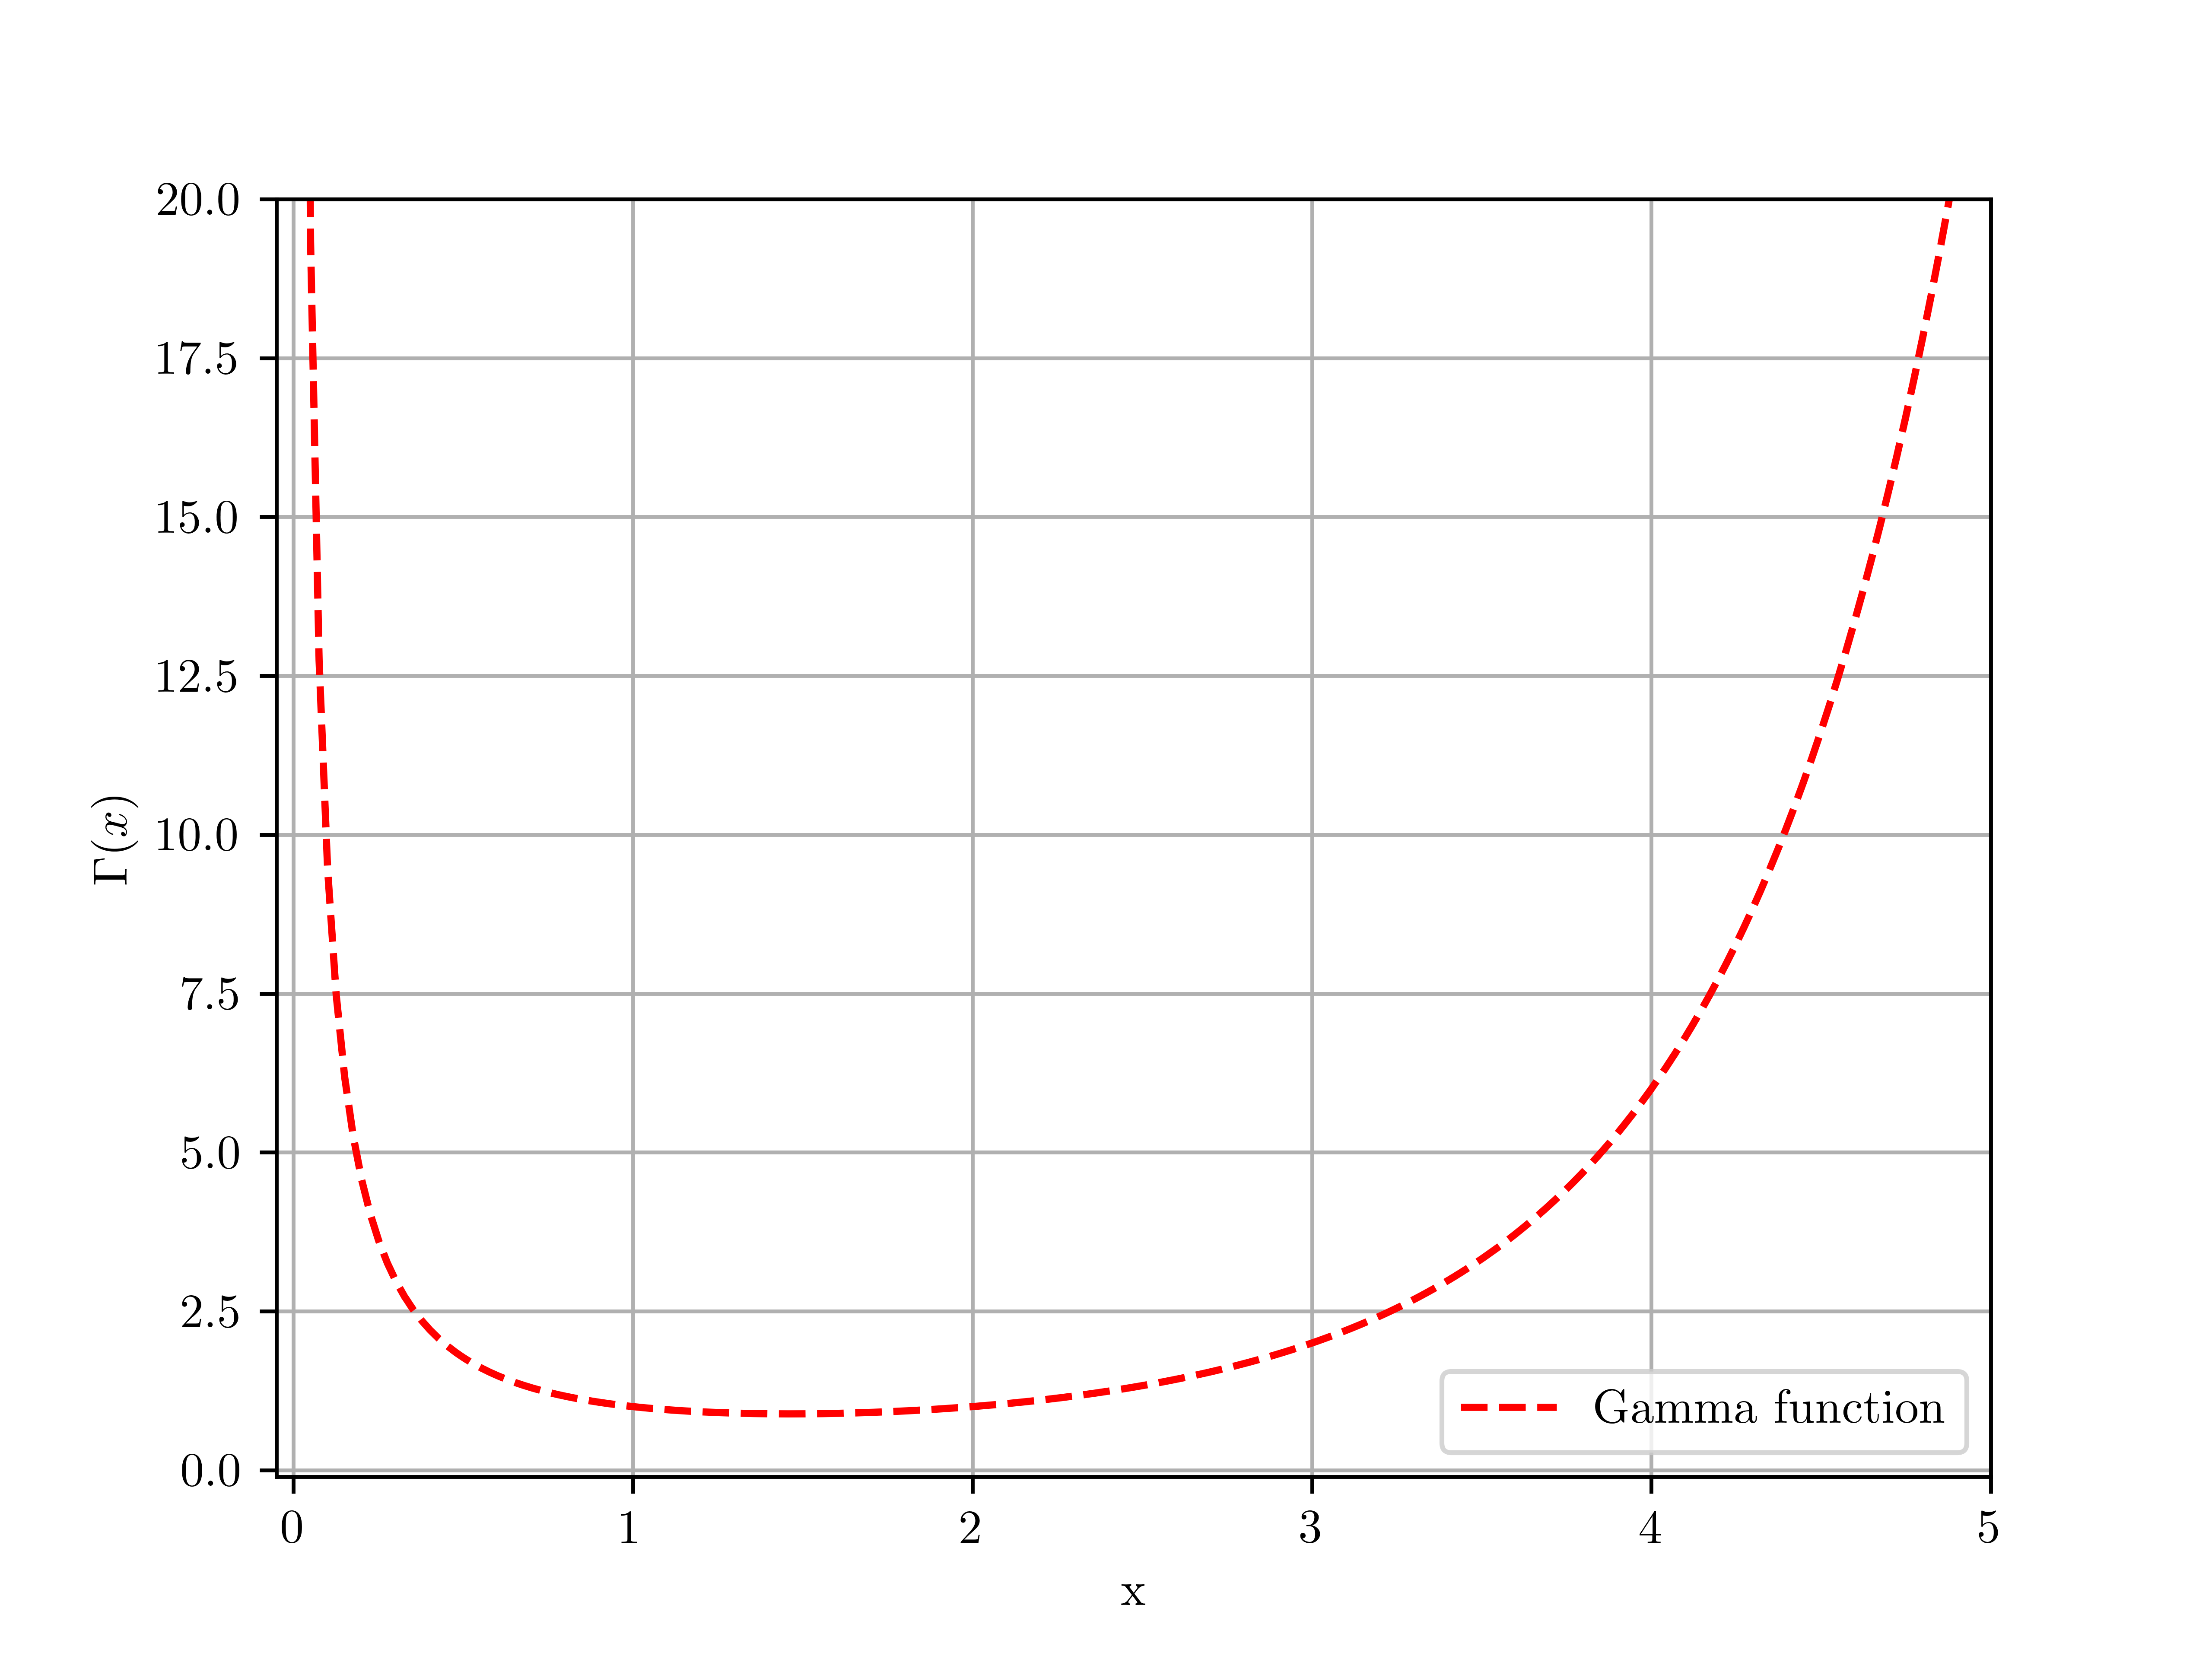
\includegraphics[scale = 0.7]{IMAGES/gamma_func.png}
    \caption{La fonction Gamma}
    \label{fig:gamma_fact}
\end{figure}
\begin{exemple}
    \begin{enumerate}
        \item $\Gamma(1) = 1$
        \item Pour $x=\frac{1}{2}$ on a 
        \begin{equation*}
            \Gamma(\frac{1}{2}) = \int_{0}^{+\infty} t^{\frac{1}{2}-1} e^{-t} dt = \int_{0}^{+\infty} t^{\frac{-1}{2} e^{-t} dt}.
        \end{equation*}
        On pose $ t = u ^ 2 $, alors $dt = 2udu$. On obtient
        \begin{equation*}
            \Gamma(\frac{1}{2}) = \int_{0}^{+\infty} t^{\frac{-1}{2}} e^{-1}dt = 2\int_{0}^{+\infty} e^{-u^2} du.
        \end{equation*}
        avec $r \in [0, +\infty[$  et $ 0  \leq \theta \leq \frac{\pi}{2}$. Alors
        \begin{align*}
            \left[\int_{0}^{+\infty} e^{{-u^2}} du\right]^2 &= \int_{0}^{+\infty} e^{-u^2} du\int_{0}^{+\infty} e^{-v^2} dv
            \\
            &= \int_{0}^{+\infty}\int_0^{+\infty} e^{-(u^2+v^2)} dudv\\ 
            &= \int_{0}^{\frac{\pi}{2}}d\theta \int_{0}^{+\infty} r e^{-r^2} dr\\
            &= \frac{\pi}{2}\left[ -\frac{1}{2} e^{-r^2}\right]_0^{+\infty} = \frac{\pi}{2}
        \end{align*}
        et par suite 
        \begin{equation*}
            \Gamma(\frac{1}{2})=\int_0^{+\infty} t^{-\frac{1}{2}} e^{-t} dt = 2\int_0^{+\infty} e^{-u^2} du = \sqrt{\pi}
        \end{equation*}
    \end{enumerate}
\end{exemple}
L'intégral d'Euler ne converge pas pour les 
$\Re(x)<0$. Mais on peut prolonger $\Gamma(x)$ (figure \ref{fig:gamma_fact}), puisque la fonction qu'elle définie dans la demi-plan complexe positive a une continuation analytique unique dans la moitié négatif du plan, on peut calculer la fonction Gamma pour les arguments positifs (\ref{gamma_tout_entiers}) en utilisant l'intégrale d'Euler, puis étendre les résultats pour inclure les nombres négatifs en utilisons la formule de récurrence de la fonction Gamma (\ref{gamma_n}).
\begin{proposition}
    Soient $n\in \mathbb{N}$. On a les identités suivantes:
        \begin{enumerate}
            \item $\Gamma(x+1) = x\Gamma(x)$, pour tout $x > 0$\label{gamma_n}
            \item $\Gamma(x+n) = x(x+1) ... (x+n-1)\Gamma(x)$, \label{gamma_tout_entiers} pour tout $x\in \mathbb{R \textbackslash Z^-}$ tel que $ -n < \Re(x) \leq -n+1 $.
        \end{enumerate}
    
\end{proposition}
\begin{proof}
    \begin{enumerate}
        \item Soit $x>0$. Nous procédons par l'usage d'une intégration par parties.\\
        \begin{align*}
            \Gamma(x+1) &= \int_{0}^{\infty} t^x e^{-t} dt \\
            &= \left[ -t^x e^{-t} \right]_0^{+\infty} + \int_{0}^{+\infty} xt^{x-1} e^{-t} dt\\ 
            &= \lim_{t \to +\infty} (-t^x e^{-x}) + x\int_{0}^{+\infty} t^{x-1}e^{-t} dt.
        \end{align*}
        Et clairement $\lim_{t \to +\infty} (t^x e^{-t}) = 0$. Donc, on en déduit par la définition de $\Gamma(x)$ que $\Gamma(x+1) = x\Gamma(x)$. \label{gamma_n}
        \item C'est une conséquence immédiate de l'identité (\ref{gamma_n}) et le principe de récurrence.
    \end{enumerate}
\end{proof}
\begin{remarque}
    Si on prend $x=1$ dans la propriété (\ref{gamma_tout_entiers}), on obtient
    \begin{equation*}
        \Gamma(n+1)=n! \hspace{1cm} \forall n \in \mathbb{N}.
    \end{equation*}
    Et cela démontre ce que nous avons dit précédemment, que le fonction gamma est la généralisation de la notion de la factorielle pour $x > 0$.
\end{remarque}
\begin{figure}[H]
    \centering
    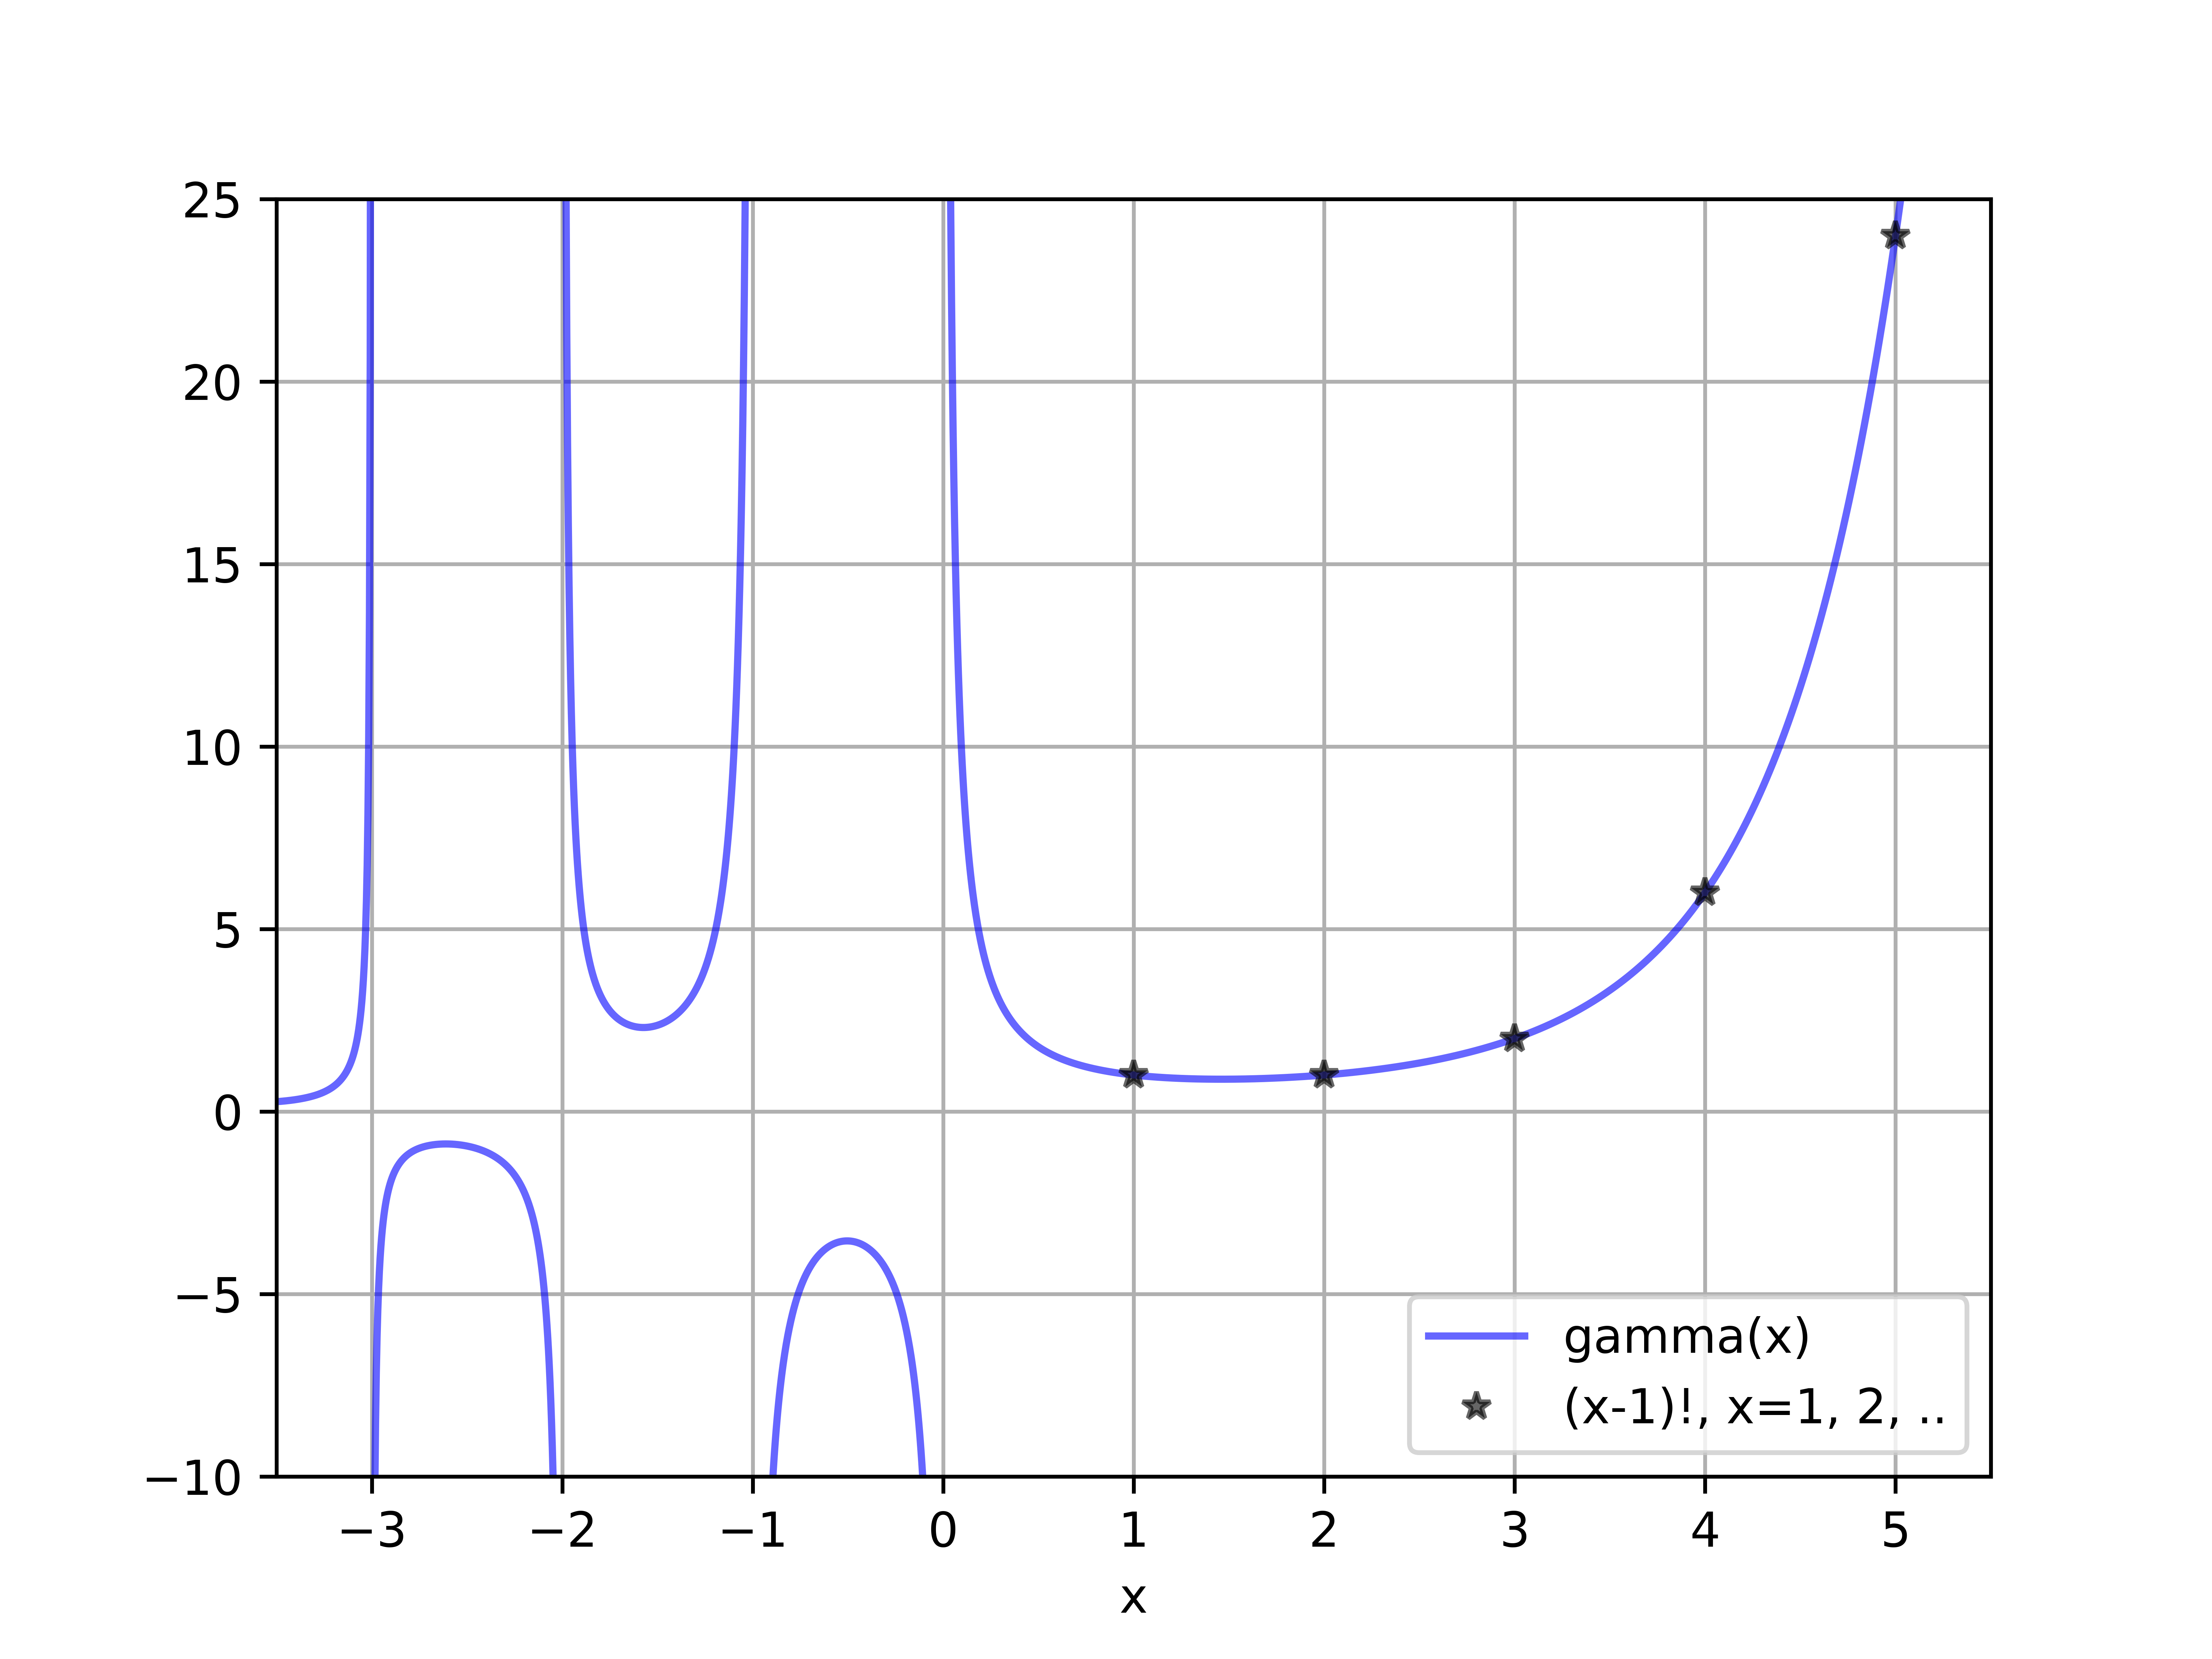
\includegraphics[scale = 0.7]{IMAGES/gamma.png}
    \caption{La relation géométrique entre la Fonction Gamma dans le domaine réel et la factorielle}
    \label{fig:gamma_fact}
\end{figure}

\begin{theoreme}
    La fonction $\Gamma$ possède les propriétés suivantes :
    \begin{enumerate}
        \item $\Gamma$ est continue sur $]0,+\infty[$.
        \item $\Gamma$ est de classe $C^{\infty}$ sur $]0, \infty[$ avec\\
        \begin{equation*}
            \Gamma^{(k)}(x) = \int_{0}^{\infty} t^{x-1}(\ln t)^k e^{-t} dt \hspace{1cm} \forall x >0, \forall k\in\mathbb{N}
        \end{equation*}
        \item $\Gamma$ est convexe.
    \end{enumerate}
\end{theoreme}
\begin{proof}
    \begin{enumerate}
        \item $f$ est continue sur $(\mathbb{R^{*+}})^2$, et pour tout $x\in \mathbb{R^{*+}}$, $f_x$ est intégrable sur $]0,+\infty[$. \\
        Montrons alors que $f$ satisfait à l'hypothèse de domination pour $x$ décrivons $[a,b]$, $a<b$, intervalle compact quelconque inclus dans $\mathbb{R^{*+}}$.\\ 
        Pour $0<t\leq 1$, $x \to t^{x-1}$ est décroissante donc pour $x\in [a,b]$, on a $0<f(x,t)\leq t^{a-1}$\\
        Pour $t\geq1$, $x\to t^{x-1}$ est croissante, et alors $x\in [a,b]$ donne $0<f(x,t)\leq e^{-t} t^{b-1}$.\\
        Soit alors $\phi:]0,+\infty[ \to \mathbb{R}$, $t \to \phi(t)$ ..\\
        $\phi$ est positive, continue par morceaux et intégrable sur$]0,+\infty[$ et 
        \begin{equation*}
            \forall(x,t)\in [a,b] \times ]0,+\infty[, \hspace{1cm} 0<f(x,t)\leq \phi(t)
        \end{equation*}
        Ainsi $\Gamma$ est continue sur $]0,+\infty[$ d'après le théorème de continuité sous le signe somme.
        \item Pour tout $k \in \mathbb{N^*}$, $f$ est de classe $C^k$ sur $(\mathbb{R^{*+}})^2$ avec \\
        \begin{equation*}
            \forall(x,t)\in(\mathbb{R^{*+}})^2, \hspace{1cm} \frac{\partial ^k f}{\partial x^k}(x,t)=(\ln t)^k e^{-t} t^{x-1}
        \end{equation*}  
        Considérons de nouveau un intervalle compact $[a,b]\subset \mathbb{R^{*+}}$ et soit $\psi _k : ]0,+\infty[ \mapsto \mathbb{R}$ telle que
        \begin{equation*}
            \forall t\in ]0,+\infty[, \hspace{1cm} \psi_k (t) = |\ln t|^k \phi(t)
        \end{equation*}
        Au voisinage de 0, on a $\psi_k (t) = o\left(\frac{1}{t^{1-\frac{a}{2}}} \right)$ et en $+\infty$, on a encore $\psi _k (t) = o\left(\frac{1}{t^2}\right)$ donc $\psi_k$ est positive, continue par morceaux et intégrale sur $]0,+\infty[$.\\
        Par construction, on a 
        \begin{equation*}
            \forall(x,t)\in[a,b]\times]0,+\infty[, \hspace{1cm} \left| \frac{\partial ^k f}{\partial x^k} (x,t) \right| \leq \psi _k(t)
        \end{equation*}
        Montrons par récurrence que pour tout $k\in\mathbb{N^*}$, $\Gamma$ est de classe $C^k$ sur $\mathbb{R^{+*}}$ avec:
        \begin{equation*}
            \mathcal{P} (k): \hspace{1cm} \forall x\in\mathbb{R^{*+}}, \Gamma^{(k)} (x) = \int_0^{+\infty} (\ln t)^k e^{-t} t^{x-1} dt
        \end{equation*}
        La classe $C^1$ de $f$ sur $(\mathbb{R^{*+}})^2$ et l'étude de la définition de $\Gamma$ assurent les premières hypothèses du théorème de dérivation sous le signe somme et les fonctions $\psi_1$ donnent l'hypothèse de domination sur tout segment $[a,b]\subset \mathbb{R^{*+}}$.(Il y a une fonction $\psi_1$ pour chaque segment $[a,b] \subset\mathbb{R^{*+}}$).\\
        Ainsi, par application du théorème, $\Gamma$ est de classe $C^1$ sur $\mathbb{R^{*+}}$ avec :
        \begin{equation*}
            \forall x\in\mathbb{R^{*+}}, \hspace{1cm} \Gamma'(x)=\int_0^{+\infty}(\ln t)e^{-t} t^{x-1}dt
        \end{equation*}
        C'est-à-dire la propriété $\mathcal{P}(1)$ est vraie.\\
        Montrons maintenant que si $\mathcal{P}(k)$ est vraie, alors $\Gamma^{(k)}$ est de classe $C^1$ sur $\mathbb{R^{*+}}$.\\
        La classe $C^{k+1}$ de $f$ sur $(\mathbb{R}^{*+})$ donne la classe $C^1$ sur $(\mathbb{R}^{*+})^2$ de $\frac{\partial ^k k}{\partial x^k}$ et $\Gamma ^{(k)}$ étant définie pour tout $x\in\mathbb{R}^{*+}$, les premières hypothèses du théorème de dérivation sous le signe somme sont vérifiées pour la fonction $g=\frac{\partial ^k f}{\partial x^k}$. D'autre part, les fonctions $\psi _{k+1}$ montrent que $\frac{\partial g}{\partial x} = \frac{\partial ^{k+1} f}{\partial x^ {k+1}}$ satisfait à l'hypothèse de domination sur tout segment $[a,b]\subset \mathbb{R}^{*+}$. On en déduit que $\Gamma ^{(k)}$ est de classe $C^1$ sur $\mathbb{R}^{*+}$, c'est-à-dire que $\Gamma$ est de classe $C^{k+1}$ avec
        \begin{equation*}
            \forall x\in \mathbb{R}^{*+}, \hspace{1cm} \Gamma^{(k+1)}(x)=\int_0^{+\infty} (\ln t)^{k+1} e^{-t} t^{x-1} dt 
        \end{equation*}
        La propriété $\mathcal{P}(k)$ est donc héréditaire, ce qui achève d'établir que $\Gamma$ est de classe $C^k$ sur $\mathbb{R}^{*+}$ pour tout $k\in \mathbb{N}^*$, donc que $\Gamma$ est de classe $C^{+\infty}$.
        \item $\Gamma ''(x) = \int_0^{+\infty} (\ln t)^2 e^{-t}t^{x-1}dt $, $\Gamma ''$ est strictement positive sur $\mathbb{R}^{*+} $ donc $\Gamma$ est convexe.
    \end{enumerate}
\end{proof}
\section{Fonction Bêta}
\begin{definition}
On désigne par $\beta(x,y)$ la fonction définie pour $x>0$ et $y>0$
par l’intégrale suivant:
    \begin{equation}
        \beta(x,y) = \int_{0}^{1} t^{x-1}(1-t)^{y-1} dt
    \end{equation}
    (première intégrale eulérienne)
\end{definition}

La fonction $\beta$ est bien définie sur $]0,+\infty[\times]0,+\infty[$.\\
Soient $(x,y)\in]0,\infty[\times]0,+\infty[:$\\
\begin{itemize}
    \item $t^{x-1}(1-t)^{y-1} \underset{t \to 0^+}{\sim} t^{x-1}$, et $0\leq \int_0^{\frac{1}{2}} t^{x-1}dt < +\infty $  car  $x>0$ donc $1-x<1$.
    \item $t^{x-1}(1-t)^{y-1}\underset{t \to{1}}{\sim}(1-t)^{y-1}$, et $0\leq\int_{\frac{1}{2}}^1 (1-t)^{y-1} dt <+\infty$ car $y>0$ donc $1-y<1$. 
\end{itemize}
Par suite $\int_0^1 t^{x-1}(1-t)^{y-1}dt$ est convergente.
\begin{figure}[H]
    \centering
    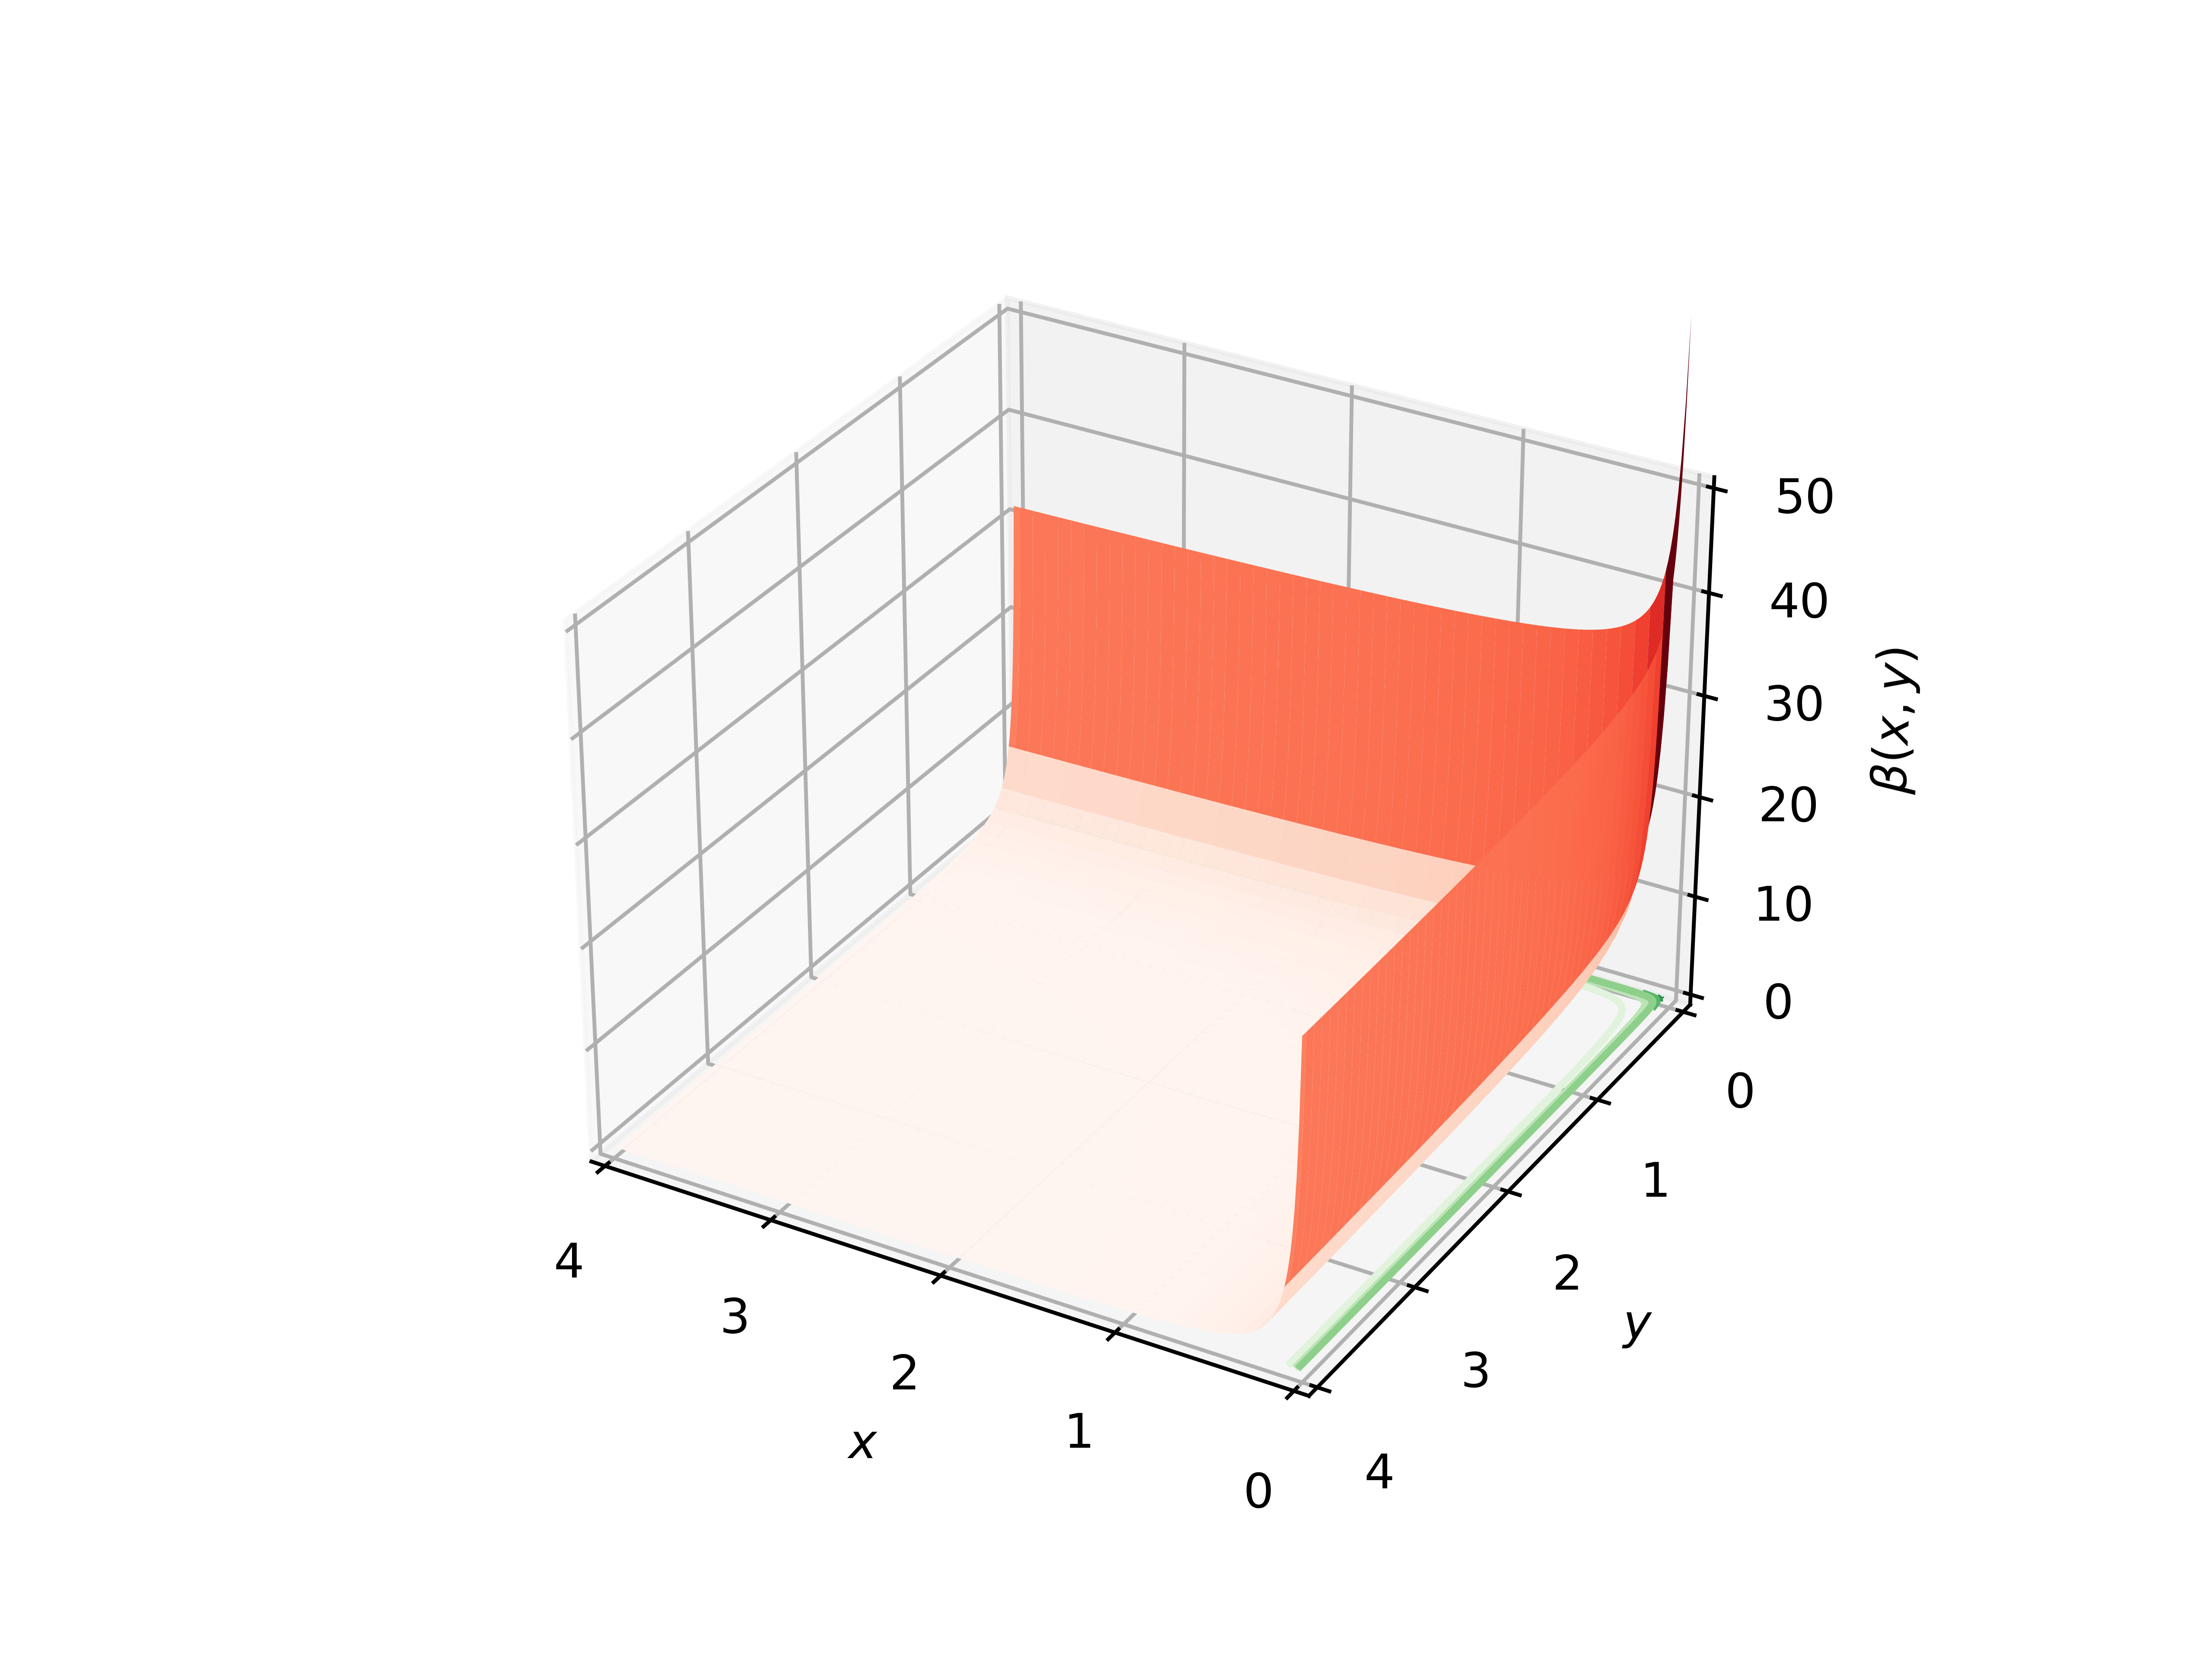
\includegraphics[scale = 0.7]{IMAGES/betaFunc.png}
    \caption{La fonction Bêta}
\end{figure}
\begin{theoreme}
    La fonction bêta est symétrique, on a
    \begin{equation}
        \beta(x,y)=\beta(y,x)
    \end{equation}
\end{theoreme}
\begin{proof}
    On considère le changement de variable $u=1-t$. Alors pour tout $x,y>0$, on a 
    \begin{equation*}
        \beta(x,y) = \int_0^1 t^{x-1}(1-t)^{y-1}dt=\int_0^1 (1-u)^{x-1} u^{y-1}du =\beta(y,x).
    \end{equation*}
\end{proof}
\begin{theoreme}
    La relation avec la fonction Gamma\\
    \begin{equation}
        \beta(x,y) = \frac{\Gamma(x)\Gamma(y)}{\Gamma(x+y)} = \frac{(x-1)!(y-1)!}{(x+y-1)!}.
    \end{equation}
\end{theoreme}
\begin{proof}
    Soit $x,y >0$, on a 
    \begin{align*}
        \Gamma(x)\Gamma(y) &= \int_0^{+\infty} e^{-t}t^{x-1}dt\int_0^{+\infty} e^{-u}u^{y-1} du\\
        &= \int_0^{+\infty}\int_0^{+\infty} e^{-(t+u)}t^{x-1}u^{y-1} dtdu \\
        &= \int_0^{+\infty}t^{x-1} dt \int_0^{\infty} e^{-(t+u)}u^{y-1}du.
    \end{align*}
    En utilisant les changements de variables $r=x+y$ et $x=rz$ avec $0\leq t\leq \infty$ et $0\leq z\leq 1$. Alors, $dx=zdr+rdz, dy=(1-z)dr-rdz$ et $dxdy=rdzdr$, donc:
    \begin{align*}
        \Gamma(x)\Gamma(y) &= \int_0^1 z^{x-1}(1-z)^{y-1}dz\int_0^{+\infty} e^{-r}r^{x+y-1}dr \\
        &= \beta(x,y)\Gamma(x+y).
    \end{align*}
    D'où 
    \begin{equation*}
        \beta(x,y)=\frac{\Gamma(x)\Gamma(y)}{\Gamma(x+y)}
    \end{equation*}
\end{proof}
\section{Fonction Mittag-Leffler}
Tout comme la fonction exponentielle $e^x$ occupe une place importante dans la théorie des équations différentielles d'ordre entier, la fonction de Mittag-Leffler, une généralisation à un seul paramètre de celle-ci, tient un rôle significatif dans le domaine des équations différentielles d'ordre fractionnaire. Définie par une série entière, la fonction de Mittag-Leffler émerge naturellement comme solution à ces équations. \cite{Mittag-Leffler}
\begin{definition}
    \begin{equation}\label{def:mittag-leffler1}
        E_{\alpha}(x) = \sum _{k=0}^{\infty} \frac{x^k}{\Gamma(\alpha k +1)}, \hspace{1cm} \alpha>0
    \end{equation}
\end{definition}
\begin{exemple}
    valeurs particulière de la fonction de Mittag-Leffler:
    \begin{enumerate}
        \item $E_0(x)=\sum_{k=0}^{\infty} \frac{x^k}{\Gamma(1)}=\sum_{k=0}^{\inf} x^k =\frac{1}{1-x}$, (somme d'une série géométrique)
        \item $E_1(x)=\sum_{k=0}^{\infty} \frac{x^k}{\Gamma(k+1)} = \sum_{k=0}^{\infty}\frac{x^k}{k!} = e^x $, (série exponentielle)
        \item $E_2(x) = \cosh(\sqrt{x})$,
        \item $E_3(x)=\frac{1}{3} \left[e^{x\frac{1}{3}} +2e^{x\frac{1}{3}} \cos(\frac{1}{2} \sqrt{3} x^{\frac{1}{3}}) \right]$,
        \item $E_4 (x) = \frac{1}{2} \left[\cos(x^{\frac{1}{4}}) + \cosh(x^{\frac{1}{4}}) \right]$.
    \end{enumerate}
\end{exemple}
\begin{figure}[H]
    \centering
    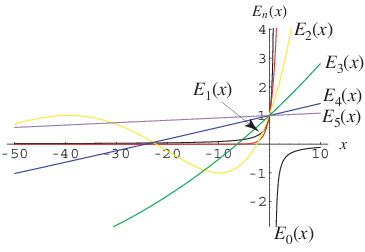
\includegraphics[scale = 0.7]{IMAGES/MittagLeffler_1001.png}
    \caption{Les fonctions de Mittag-Leffler \cite{plot:mittag-leffler}}
\end{figure}
La fonction de Mittag-Leffler à deux paramètres $E_{\alpha,\beta}$ généralisant la définition précédente \ref{def:mittag-leffler1}
\begin{definition}
définie par le développement en série suivant:
    \begin{equation}\label{def:mittag-leffler2}
        E_{\alpha, \beta}(x) = \sum _{k=0}^{\infty} \frac{x^k}{\Gamma(\alpha k +\beta)}, \hspace{1cm} \alpha>0, \hspace{0.3cm}\beta>0
    \end{equation}
\end{definition}
la série converge pour toute valeur d'argument x, c qui fait de la fonction une fonction entière.
\begin{remarque}
    Si $\beta =1$, alors $E_{\alpha, \beta}$ coïncide avec $E_{\alpha}$
    \begin{equation}
        E_{\alpha, 1}=E_{\alpha}
    \end{equation}
\end{remarque}
\begin{exemple}
    pour x proche de zéro, nous obtenons
    \begin{enumerate}
        \item $E_{1,1} (x)=\sum_{k=0}^{\infty} \frac{x^k}{\Gamma(k+1)} = \sum_{k=0}^{\infty} \frac{x^k}{k!} = e^x$,
        \item $E_1,2(x) = \sum_{k=0}^{\infty} \frac{x^k}{\Gamma(k+2)} = \sum_{k=0}^{\infty} \frac{x^k}{(k+1)!} = \frac{1}{x} \sum_{k=0}^{\infty} \frac{x^{k+1}}{(k+1)!} = \frac{e^x - 1}{x}$
    \end{enumerate}
\end{exemple}
\begin{remarque}
    Les fonctions hyperboliques $\sinh$ et $\cosh$ sont aussi des cas particuliers de la fonction de Mittag-Leffler à deux paramètres
    \begin{enumerate}
        \item $E_{2,1} (x^2) = \sum_{k=0} ^{\infty} \frac{x^{2k}}{\Gamma(2k +1)} = \sum_{k=0}^{\infty} \frac{x^{2k}}{(2k)!} = \cosh(x)$,
        \item $E_{2,2}(x^2) = \sum_{k=0}^{\infty} \frac{x^{2k}}{\Gamma(2k+2)} = \frac{1}{x}\sum_{k=0}^{\infty} \frac{x^{2k+1}}{\Gamma(2k+1)!} = \frac{\sinh(x)}{x} $.
    \end{enumerate}
\end{remarque}
\begin{theoreme}
    la fonction de Mittag-Leffler satisfait la formule de différenciation suivante:
    \begin{equation}
        \left(\frac{d}{dx} \right)^n \left[x^{\beta-1}E_{n,\beta}(\lambda x^n) \right] = x^{\beta-n-1} E_{n,\beta-n}(\lambda x^n), \hspace{1cm} (n\in \mathbb{N}, \lambda \in \mathbb{C}).
    \end{equation}
\end{theoreme}


% CHAPITRE II
%%%%%%%%%%%%%%%%%%%%%%%%%%%%%%%%%%%%%%%%%%%%%%%%%%
%%%%		~~~~ Method ~~~~
%%%%%%%%%%%%%%%%%%%%%%%%%%%%%%%%%%%%%%%%%%%%%%%%%%


\chapter{Éléments du calcul fractionnaire}
\label{chap:Dérivées et Intégrales d'ordre non entier}
\pagestyle{fancy}
\section{Intégrale fractionnaire au sens de Riemann-Liouville} 
\subsection{Définition}
L'approche de Riemann-Liouville offre une perspective solide et intuitive sur l'intégration fractionnaire. Cette méthode est basée sur la formule de Cauchy pour le n-ème intégral qui utilise seulement une simple intégration.
\begin{equation} \label{eq:int_succ}
    I_{a}^{n} f(t) = \int_{a}^{t} \int_{a}^{\tau_{n-1}} ... \int_{a}^{\tau_1} f(\tau) d\tau d\tau_1 ... d\tau_{n-1} = \frac{1}{(n-1)!}\int_{a}^{t} (t-\tau)^{n-1} f(\tau)d\tau
\end{equation}
\begin{proof}
    Par récurrence, le cas où $ n= 1$ est évidemment vérifié. Ainsi, nous allons montrer le cas où $n=2$.
    On a 
    \begin{align*}
    \frac{1}{1!} \int_{a}^{t} (t - \tau) f(\tau) d\tau &= \left|^{u = t-\tau}_{v'= f(\tau)} \hspace{0.5cm} {_{v = \int_{a}^{\tau} f(r) dr} ^{u'=-1}}\right| \\
    &= \left[(t-\tau)\int_{a}^{\tau}f(r)dr \right]_{\tau=a}^{\tau=t} + \int_{a}^{t}\int_{a}^{\tau}f(r)dr = {}_{a}I_t^2 f(t)
    \end{align*}
    
    En effet, à la limite supérieure, le polynôme est nul, tandis qu'à la limite inférieure, nous intégrons sur un ensemble de mesure nulle.\\
    Nous supposons maintenant que la formule est valide pour $n$ général. Nous procédons alors à une intégration supplémentaire $n+1$
    \begin{align*}
        \int_{a}^{t} I_{a}^{n} f(r)dr &= \int_{a}^{t}  \frac{1}{(n-1)!} \int_{a}^{r} (r - \tau)^{n-1} f(\tau) d\tau dr \\
        &= \frac{1}{(n-1)!} \int_{a}^{t}f(\tau)\int_{\tau}^{t} (r - \tau)^{n-1} drd\tau
        = \frac{1}{(n-1)!} \int_{a}^{t}f(\tau) \left[ \frac{(r-\tau)^n}{n} \right]_\tau ^t d\tau \\
        &= \frac{1}{n!} \int_{a}^{t} (t-\tau)^n f(\tau) d\tau \\
        &= I_a^{n+1} f(t)
    \end{align*}
\end{proof}
Puisque la fonction Gamma prolonge la fonction factorielle à l'ensemble des nombres réels, nous pouvons remplacer l'entier $n$ par le nombre réel positif $\alpha$, dans \ref{eq:int_succ}, alors nous obtenons la définition suivante:
\begin{definition}
    L'intégrale fractionnaire de Riemann-Liouville d'ordre $\alpha \in \mathbb{R^+}$ d'une fonction $f\in \textbf{L}^1 [a,b]$ est définie par:
    \begin{equation}\label{eq:integraleR-L}
        I_{a}^{\alpha} f(t) = {}_a^{RL} D_t^{-\alpha} f(t) =\frac{1}{\Gamma(\alpha)} \int_{a}^{t} (t-s)^{\alpha-1} f(s) ds.
    \end{equation}
\end{definition}
L'intégrale fractionnaire $I_a^{\alpha} f$ peut être réécrite sous la forme :
\begin{equation}
    I_{a}^{\alpha} f(t) = \frac{1}{\Gamma(\alpha)} \int_{0}^{t-a} s^{\alpha -1}f(t-s)ds, \hspace{1cm} t\in[a,b].
\end{equation}
Nous aboutissons donc au théorème suivant:
\begin{theoreme}
    Soient $f\in \textbf{L}^1 [a,b]$ et $\alpha > 0$. Alors, l'intégrale fractionnaire $I_a^{\alpha}$ existe pour tout $t\in[a,b]$ et la fonction $I_a^{\alpha} f$ est un élément de $\textbf{L}^1 [a,b]$. 
\end{theoreme}
\subsection{Intégrales fractionnaires au sens de R-L de quelques fonctions usuelles}
\subsubsection*{Fonction puissance} 
Soit la fonction $f(t)=(t-a)^\beta$, \hspace{0.3cm} $t\in[a,b]$, \hspace{0.3cm} $a\in\mathbb{R}$ \hspace{0.3cm} et $\beta > -1$. \\
Par la relation \ref{eq:integraleR-L} on a:
\begin{equation*}
    I_{a}^{\alpha} (t-a)^\beta=\frac{1}{\Gamma(\alpha)} \int_{a}^{t}(t-s)^{\alpha - 1} (s-a)^{\beta}ds
\end{equation*}
    et par le changement de variable $\tau = a + (t-a)s$, on obtient
    \begin{align*}
         I_{a}^{\alpha} (t-a)^{\beta} &= \frac{(t-a)^{\beta+\alpha}}{\Gamma(\alpha)} \int_0^1 s^{\beta - 1 + 1}(1-s)^{\alpha - 1}\\
         &= \frac{(t-a)^{\beta + \alpha}}{\Gamma(\alpha)} B(\alpha, \beta +1)\\
         &= \frac{(t-a)^{\beta + \alpha}}{\Gamma(\alpha)} \frac{\Gamma(\alpha)\Gamma(\beta + 1)}{\Gamma(\beta + \alpha + 1)}
\end{align*}
alors  l'intégral fractionnaire au sens de Riemann-Liouville de $f$ est donné par
\begin{equation} \label{eq:I_R-L_fct_puissance}
    I_{a}^{\alpha} (t-a)^\beta=\frac{\Gamma(\beta +1)}{\Gamma(\beta + \alpha + 1)}(t-a)^{\beta + \alpha}.
    \end{equation}

\begin{exemple}
En particulier, de \ref{eq:I_R-L_fct_puissance} si $a=0$, on a
\begin{equation*}
    I_{0}^{\alpha} (t)^{\beta} = \frac{\Gamma(\beta + 1)}{\Gamma(\beta + \alpha + 1)}t^{\beta + \alpha}
\end{equation*}
    et si $\alpha = \frac{1}{2}$ et $a = 0$, on a 
    \begin{enumerate}
        \item $I_0^{\frac{1}{2}}t^0=\frac{\Gamma(1)}{\Gamma(\frac{3}{2})} t^{\frac{1}{2}} = 2\sqrt{\frac{t}{\pi}}$
        \item $I_0^{\frac{1}{2}} t^1=\frac{\Gamma(2)}{\Gamma(\frac{5}{2})} t^{\frac{3}{2}} = \frac{4}{3}\sqrt{\frac{t^3}{\pi}}$
        \item $I_0^{\frac{1}{2}} t^2  =\frac{\Gamma(3)}{\Gamma(\frac{7}{2})} t^{\frac{5}{2}} = \frac{16}{15}\sqrt{\frac{t^5}{\pi}}$
    \end{enumerate}
\end{exemple}
\subsubsection*{Fonction constante} 
Soit $f(t) =C \in \mathbb{R}$ est une constante. Alors 
\begin{equation} \label{integral_R-L}
    I_{a}^{\alpha} C= \frac{C}{\Gamma(\alpha + 1)}(t-a)^\alpha
\end{equation}
\begin{exemple}
    Soit $f$ la fonction définie sur $\mathbb{R}$ par : $f(t) = 1$\\
    \begin{equation*}
        I_a^{\alpha}(1) = \frac{(t-a)^\alpha}{\Gamma(\alpha + 1)}
    \end{equation*}
\end{exemple}
\subsubsection*{Fonction exponentielle} Soit $f(t) = e^{kt}$, où $k\in \mathbb{R}$ est une constante, alors par la \ref{eq:I_R-L_fct_puissance} on a :
\begin{equation*}
     I_{a}^{\alpha} e^{kt}=\frac{1}{\Gamma(\alpha)} \int_{a}^{t} (t-s)^{\alpha - 1}e^{ks}ds
\end{equation*}
En faisant le changement de variable $s=t-\tau$, on obtient
\begin{equation*}
    I_{a}^{\alpha} e^{kt}=\frac{1}{\Gamma(\alpha)} \int_{0}^{t-a} s^{\alpha - 1} e^{k(t-s)}ds
\end{equation*}
Alors l'intégrale fractionnaire au sens de Riemann-Liouville de $f$ est donnée par:
\begin{equation}\label{eq:I_R-L_f_expo}
    I_{a}^{\alpha} e^{kt}=\frac{1}{\Gamma(\alpha)} \int_{0}^{t-a} s^{\alpha - 1}e^{k(t-s)} ds.
\end{equation}
\subsection{Quelques propriétés de base}
    La formule \ref{eq:integraleR-L} représente l'intégrale d'ordre arbitraire $\alpha > 0$, mais ne permet pas l'ordre $\alpha = 0$ qui correspond formellement à l'opérateur d'identité. \\
    Si la fonction $f$ est continue pour $t \geq a$, alors on considère la limite : $\lim_{\alpha\to 0^+} (I_{a}^{\alpha}f)(t) = f(t)$ \cite{FDEs_intro}.\\
    par conséquent nous pouvons écrire $I_a^0 f(t)=f(t)$ \\
\heading{Composition des intégrales fractionnaires}
L'opérateur intégral fractionnaire de Riemann-Liouville vérifie la propriété suivante:
\begin{proposition}
    Soient $f \in C[a,b]$ $\beta >0$, et $\alpha >0$. Alors on a 
    \begin{equation}
        I_{a}^{\alpha}[I_{a}^{\beta}f(t)] = I_{a}^{\alpha + \beta} f(t)
    \end{equation}
\end{proposition}
\begin{proof}
La preuve découle directement de la définition \ref{eq:integraleR-L}:
    \begin{align*}
        I_a^{\alpha}[I_a^{\beta}f(t)] &= I_a^{\alpha}[\frac{1}{\Gamma(\beta)} \int_{a}^{t} (t-s)^{\beta-1} f(s) ds] = I_a^{\alpha}[g(s)ds]\\
        &= \frac{1}{\Gamma(\alpha)} \int_{a}^{\tau} (\tau - u)^{\alpha - 1} [g(u) du] \\
        &= \frac{1}{\Gamma(\alpha)} \int_{a}^{\tau} (\tau - u)^{\alpha - 1} \left[\frac{1}{\Gamma(\beta)} \int _{a}^{t} (t-u)^{\beta - 1} f(u)du\right] \\
        &= \frac{1}{\Gamma(\alpha) \Gamma(\beta)} \int_{a}^{\tau} (\tau - t) \int_{a}^{t}(t-u)^{\beta - 1} f(u)du\\
    \end{align*}
    et par le changement de variable $ t = u + (\tau - u)$ on obtient:\\
    \begin{align*}
        I_{a}^{\alpha}[I_{a}^{\beta}f(t)] = \frac{\beta(\alpha, \beta)}{\Gamma(\alpha) \Gamma(\beta)} \int_{a}^{\tau} (\tau - t)^{\alpha + \beta - 1} f(u) du = I_{a}^{\alpha + \beta} f(t)
    \end{align*}
\end{proof}

\begin{proposition}
    Pout tout $\alpha, \beta >0$ et $f$ Lebesgue-intégrable sur $[a,b]$ on a :
    \begin{equation}
        \frac{d^k}{dt^k}[I_a^{\alpha} f(t)] = I_{a}^{\alpha - k} f(t) , \alpha >1, \hspace{1cm}\forall k <\alpha.
    \end{equation}
\end{proposition}
\begin{remarque}
    En générale: $D[_{a}I_t^{\alpha}f(t)] \neq {}_{a}I_t^{\alpha} [D f(t)]$ et alors on a le théorème suivant:
\end{remarque}
\begin{theoreme}
    Soient $f$ fonction continue sure $[0,b[$. Si $Df$ est continue alors pour tout $t>0$ on a :
    \begin{equation}
        D[I_{t}^{\alpha}f(t)] = I_{t}^{\alpha}[Df(t)]+\frac{f(0)}{\Gamma(\alpha)}t^{n-\alpha}
    \end{equation}
\end{theoreme}

\section{Dérivée fractionnaire au sens de Riemann-Liouville}
\subsection{Définition}
Tout d'abord, rappelons que pour tout fonction $f$ ayant une dérivée d'ordre $n$ continue sur l'intervalle $[a,b]$, nous avons:
\begin{equation}\label{eq:def_R-L}
    D^n = D^m I^{m-n} f,
\end{equation}
où $n,m\in\mathbb{N}$, tel que $m>n$. \\
Supposons que $n$ n'est pas un entier. Nous arrivons à la définition de l'opérateur différentiel fractionnaire de Riemann-Liouville. Cependant, il n'existe pas d'équivalent pour la n-ème dérivée comparable à \ref{eq:int_succ}, ce qui nous oblige à généraliser les dérivées via une intégrale fractionnaire. Initialement, nous introduisons une perturbation de l'ordre entier à l'aide d'une intégrale fractionnaire selon \ref{integral_R-L}, puis nous employons un nombre approprié de dérivées conventionnelles. \cite{FDE&applications}
\begin{definition}
    La dérivée fractionnaire au sens de Riemann-Liouville d'ordre $\alpha$ de la fonction $f$, notée $ \textbf{D}_a^{\alpha}$, est la fonction définie par :\\
    \begin{equation} \label{eq:D_R-L}
        \textbf{D}_a^{\alpha} = \frac{d^n}{dt^n} \left[I_a^{n-\alpha} f(t) \right],
    \end{equation}
    avec $n =[\alpha] + 1$ où $[.]$ est la partie entière. 
\end{definition}
De manière équivalente, nous avons:
\begin{equation}
    \textbf{D}_a^{\alpha} =
    \begin{cases}
        \frac{1}{\Gamma(n-\alpha)} \frac{d^n}{dt^n}\left( \int_a^t(t-s)^{n-\alpha-1}f(s)ds\right) \hspace{1cm} n-1<\alpha<n, \hspace{0.3cm} n\in\mathbb{N^*}\\
        \frac{d^n}{dt^n} f(t), \hspace{1cm} \alpha =n.
    \end{cases}
\end{equation}
\subsection{Dérivées fractionnaires de quelques fonctions usuelles}
\subsubsection*{Fonction puissance} 
Soient la fonction $g(t)=(t-a)^\gamma$, et $0<n-1<\alpha<n$ avec $\gamma > n-1$ on a alors: 
\begin{equation*}
    \textbf{D}_a^{\alpha} (t-a)^{\gamma} = \frac{1}{\Gamma(n-\alpha)} \frac{d^n}{dt^n} \int_a^t(t-\tau)^{n-\alpha-1} (\tau -a)^{\gamma} d\tau
\end{equation*}
    et par le changement de variable $\tau = a + (t-a)s$, on obtient
    \begin{align*}
         \textbf{D}_a^{\alpha} (t-a)^{\gamma} &= \frac{1}{\Gamma(n- \alpha)} \frac{d^n}{dt^n} (t-a)^{n+\gamma-\alpha} \int_0^1 (1-s)^{n-\alpha -1} s^{\gamma}ds\\
         &= \frac{\Gamma(n+\gamma-\alpha+1)B(n-\alpha,\gamma+1)}{\Gamma(n-\alpha)\Gamma(\gamma-\alpha +1)}(t-a)^{\gamma-\alpha}\\
         &= \frac{\Gamma(n+\gamma-\alpha+1)\Gamma(n-\alpha)\Gamma(\gamma +1)}{\Gamma(\gamma-\alpha +1)\Gamma(n-\alpha)\Gamma(n+\gamma-\alpha+1)}(t-a)^{\gamma-\alpha}\\
         &= \frac{\Gamma(\gamma+1)}{\Gamma(\gamma - \alpha +1)}(t-a)^{\gamma - \alpha}
\end{align*}
\begin{exemple}
Pour $\alpha = \frac{1}{2}, \gamma=\frac{1}{2}, a= 0$, nous aurons
\begin{equation*}
    \textbf{D}_a^{\frac{1}{2}} t^{\frac{1}{2}} = \frac{\Gamma(\frac{3}{2})}{\Gamma(1)}= \Gamma(\frac{3}{2}) 
\end{equation*}
\end{exemple}
\subsubsection*{Fonction constante} 
Soit $g(t) =C \in \mathbb{R}$ est une constante. Alors 
\begin{equation}
    \textbf{D}_a^{\alpha} C=\frac{C}{\Gamma(1-\alpha)}(t-a)^{-\alpha}.
\end{equation}
\subsection{Quelques Propriétés de base} 



\heading{Linéarité}

Soient $\lambda, \gamma\in \mathbb{R}$. D'après la définition de la dérivée fractionnaire de Riemann-Liouville, il vient que:
\begin{equation}
    \textbf{D}_a^{\alpha}(\lambda f(t) + \gamma g(t)) = \lambda\textbf{D}_a^{\alpha} f(t) +\gamma\textbf{D}_a^{\alpha} g(t).
\end{equation}
En effet,
\begin{align*}
    \textbf{D}_a^{\alpha}(\lambda f(t) + \gamma g(t)) &=  \frac{1}{\Gamma(n-\alpha)} \frac{d^n}{dt^n}\int_a^t (t-s)^{n-\alpha-1}(\lambda f(s)+\gamma g(s))ds\\
    &= \frac{\lambda}{\Gamma(n-\alpha)} \frac{d^n}{dt^n}\int_a^t(t-s)^{n-\alpha-1}f(s) ds +\frac{\gamma}{\Gamma(n-\alpha)} \frac{d^n}{dt^n}\int_a^t(t-s)^{n-\alpha-1}g(s)ds\\
    &=\lambda \textbf{D}_a^{\alpha} f(t) +\gamma\textbf{D}_a^{\alpha} g(t).
\end{align*}
\heading{Composition à droite avec intégrale fractionnaire}
Pour $\alpha>0$ et $t>a$, nous avons :
\begin{equation}
    \textbf{D}_a^{\alpha}\left(I_a^{\alpha}f(t)\right) = f(t)
\end{equation}
C'est-à-dire que l'opérateur de dérivation fractionnaire au sens de Riemann-Liouville est un inverse gauche de l'opérateur d'intégration fractionnaire
\begin{itemize}
    \item Cas où $\alpha=k\in\mathbb{N^*}$:\\
    \begin{align*}
        \textbf{D}_a^{\alpha}\left(I_a^{\alpha}f(t)\right) &= \frac{1}{\Gamma(n)}\frac{d^k}{dt^k}\int_a^t (t-a)^{k-1} f(s) ds\\
        &=\frac{d}{dt}\int_a^tf(s)ds\\
        &=f(t)
    \end{align*}
    \item Cas où $n-1\leq \alpha<n,  n\in\mathbb{N^*}$:\\
    Nous savons que :
    \begin{equation*}
        \left(I_a^{n-\alpha}(I_a^{\alpha}f(t)) \right) = I_a^nf(t)
    \end{equation*}
    et que :
    \begin{equation*}
         \textbf{D}_a^{\alpha}f(t) =  \frac{d^n}{dt^n} \left(I_a^{n-\alpha} f(t)\right)
    \end{equation*}
    Nous avons alors:
    \begin{align*}
        \textbf{D}_a^{\alpha}\left(I_a^{\alpha} f(t)\right) &= \frac{d^n}{dt^n} \left(I_a^{n-\alpha}(I_a^{\alpha}) f(t)\right)\\
        &= \frac{d^n}{dt^n}I_a^nf(t)\\
        &= f(t).
    \end{align*}
\end{itemize}
\heading{Composition à droite avec intégrale fractionnaire d'ordre différent}
Pour $\alpha \geq 0$ et $\beta \geq 0$, nous avons
\begin{equation*}
    \textbf{D}_a^{\alpha}\left(I_a^{\beta} f(t)\right) = \textbf{D}_a^{\alpha - \beta} f(t)
\end{equation*}
où $f$ est une fonction continue et que $\textbf{D}_a^{\alpha-\beta}f$ existe si $\alpha \geq \beta$.\\
Si $\alpha - \beta<0$, alors:
\begin{equation}
    \textbf{D}_a^{\alpha - \beta} f(t) = I_a^{\beta-\alpha}f(t).
\end{equation}
En effet,
\begin{itemize}
    \item Si $\beta \geq \alpha \geq 0$, nous avons :
    \begin{align*}
        \textbf{D}_a^{\alpha}\left(I_a^{\beta} f(t)\right) &= \textbf{D}_a^{\alpha}\left(I_a^{\alpha} I_a^{\beta-\alpha} f(t)\right)\\
        &= I_a^{\alpha - \beta} f(t)
    \end{align*}
    \item Si $\alpha>\beta\geq0$, nous avons:\\
    Pour $n$ et $m$ deux entiers tels que : $0\leq n-1 \leq \alpha < n$ et $0\leq m-1\leq\alpha - \beta<m$,
    \begin{align*}
        \textbf{D}_a^{\alpha}\left(I_a^{\beta} f(t)\right) &= \frac{d^n}{dt^n}\left(I_a^{n-\alpha}\left(I_a^{\beta} f(t)\right)\right)\\
        &= \frac{d^n}{dt^n}\left(I_a^{n-\alpha+\beta} f(t)\right)\\
        &= \frac{d^m}{dt^m}\left(I_a^{m-\alpha+\beta} f(t)\right)\\
        &= \textbf{D}_a^{\alpha - \beta} f(t)
    \end{align*}
\end{itemize}
\begin{remarque}
    Dans le cas des dérivées fractionnaires, la loi de composition ne peut pas être généralisée sans imposer des restrictions supplémentaires sur $f$. Elle n'est pas nécessairement vérifiée pour tout $\alpha$ et $\beta$. Nous allons énoncer précisément les conditions dans lesquelles cette loi s'applique.
\end{remarque}
\heading{Composition avec les dérivées d'ordre entier}
La composition de la dérivée fractionnaire de Riemann-Liouville avec la dérivée d'ordre entier apparaît dans de nombreux problèmes appliqués, il et donc pratique de l'introduire ici.\\
Pour $n \leq n-1 \leq \alpha < n$, $n\in \mathbb{N^*}$,
\begin{equation}
    \frac{d^k}{dt^k} \left( \textbf{D}_a^{\alpha} f(t) \right) = \textbf{D}_a^{k+\alpha} f(t),
\end{equation}
\begin{equation}\label{eq:composition_d_n}
    \textbf{D}_a^{\alpha}\left(\frac{d^k}{dt^k}f(t) \right)=\textbf{D}_a^{k+\alpha}f(t) - \sum _{i=1}^{k-1}\frac{f^{(i)}(a) (t-a)^{i-\alpha -k}}{\Gamma(i-\alpha-k+1)}.
\end{equation}
En effet, d'après la relation \ref{eq:D_R-L}, nous avons:
\begin{align*}
    \frac{d^k}{dt^k} \left( \textbf{D}_a^{\alpha} f(t) \right) &= \frac{1}{\Gamma(n-\alpha)} \frac{d^{n+k}}{dt^{n+k}} \int_a^t (t-s)^{n-\alpha-1} f(s)ds,\\
    &= \frac{1}{\Gamma((n+k)-(\alpha +k))} \frac{d^{n+k}}{dt^{n+k}}\int _a^t (t-s)^{(n+k)-(\alpha +k)-1}f(s)ds\\
    &= \textbf{D}_a^{k+\alpha} f(t),
\end{align*}
avec $(n+k-1\leq \alpha + k <n+k)$.
Pour l'égalité \ref{eq:composition_d_n}, nous avons d'après la formule \ref{eq:int_succ}:
\begin{align*}
    I_a^k f^{(k)} &= \frac{1}{(k-1)!}\int_a^t (t-s)^{k-1} f^{(k)} (s) ds,\\
    &= f(t) -\sum_{i=1}^{k-1} \frac{f^{(i)} (a) (t-a)^i}{\Gamma(i+1)}.
\end{align*}
Par conséquent, 
\begin{align*}
    \textbf{D}_a^{\alpha} \left(\frac{d^k}{dt^k}f(t) \right) = \textbf{D}_a^{\alpha}\left(f^{(k)}(t) \right),\\
    &= \textbf{D}_a^{\alpha+k} \left(I_a^k f^{(k)}(t) \right),\\
    &= \textbf{D}_a^{\alpha +k} \left(f(t) -\sum_{i=1}^{k-1} \frac{f^{(i)}(a)(t-a)^i}{\Gamma(i+1)} \right),\\
    &= \textbf{D}_a^{\alpha +k} f(t) -\sum_{i=1}^{k-1} \frac{f^{(i)}(a)(t-a)^{i-\alpha-n}}{\Gamma(i-\alpha -n +1)}.\\
\end{align*}
\heading{Composition avec les dérivées fractionnaires}
Pour $n-1\leq \alpha <n$ et $m-1\leq \beta <m$, nous avons:
\begin{equation}
    \textbf{D}_a^{\alpha} \left(\textbf{D}_a^{\beta} f(t) \right) = \mathbf{D}_a^{\alpha+\beta}f(t) -\sum_{i=1}^m [\textbf{D}_a^{\beta -i} f(t)]_t=a \frac{(t-a)^{-\alpha-i}}{\Gamma(-\alpha -i +1)},
\end{equation}
et
\begin{equation}
        \textbf{D}_a^{\beta} \left(\textbf{D}_a^{\alpha} f(t) \right) = \mathbf{D}_a^{\beta+\alpha}f(t) -\sum_{i=1}^n [\textbf{D}_a^{\alpha -i} f(t)]_{t=a} \frac{(t-a)^{-\beta-i}}{\Gamma(-\beta -i +1)},
\end{equation}
En effet, d'après la relation \ref{eq:def_R-L}, nous avons:
\begin{equation*}
    \textbf{D}_a^{\alpha} \left(\textbf{D}_a^{\beta} f(t)\right) = \frac{d^n}{dt^n} \left(I^{n-\alpha}(\textbf{D}_a^{\beta} f(t))\right)
\end{equation*}
Donc, nous aurons:
\begin{equation*}
    \textbf{D}_a^{\alpha}(\textbf{D}_a^{\beta} f(t)) = \frac{d^n}{dt^n} \left(\textbf{D}_a^{\alpha+\beta-n} f(t) -\sum_{i=1}^m [\textbf{D}_a^{\beta -i} f(t)]_ {t=a} \right) = \frac{(t-a)^{n-\alpha-i}}{\Gamma(n-\alpha-i+1)},
\end{equation*}
par la suite, nous avons:
\begin{equation*}
    \textbf{D}_a^{\alpha}(\textbf{D}_a^{\beta} f(t))=\textbf{D}_a^{\alpha+\beta} f(t) -\sum_{i=1}^m[\textbf{D}_a^{\beta-i}f(t)]_{t=a} \frac{(t-a)^{-\alpha-i}}{\Gamma(-\alpha-i+1)},
\end{equation*}
De meme pour:
\begin{equation*}
    \textbf{D}_a^{\beta}(\textbf{D}_a^{\alpha} f(t)) = \textbf{D}_a^{\beta+\alpha} f(t) -\sum_{i=1}^n[\textbf{D}_a^{\alpha-i}f(t)]_{t=a} \frac{(t-a)^{-\beta-i}}{\Gamma(-\beta -i+1)}.
\end{equation*}
En général, les opérateurs de dérivation fractionnaire, au sens de Riemann-Liouville, ne commutent pas. Mais, nous avons la propriété essentielle suivante:
\begin{equation}
    \textbf{D}_a^{\alpha}\left(\textbf{D}_a^{\beta} f(t)\right) = \textbf{D}_a^{\beta} \left( \textbf{D}_a^{\alpha} f(t)\right) = \textbf{D}_a^{\alpha+\beta}f(t),
\end{equation}
si et seulement si: \\
\begin{equation}
    \begin{cases}
        \textbf{D}_a^{\alpha -i} f(t)|_{t=a} =0, \hspace{1cm} i=1,2,...,n,\\
        \textbf{D}_a^{\beta -j} f(t)|_{t=a}=0, \hspace{1cm} j=1,2,...,m.
    \end{cases}    
\end{equation}
\section{Dérivée fractionnaire au sens de Caputo}
Avant de présenter la définition, il est important de souligner les similitudes structurelles avec la dérivée de Riemann-Liouville. Tout comme la dérivée de Riemann-Liouville utilise une intégrale fractionnaire pour capturer les comportements passés d'une fonction, la dérivée de Caputo utilise également une intégrale fractionnaire pour prendre en compte les valeurs passées. Cependant, la différence majeure réside dans l'ordre de différentiation, où la dérivée de Caputo permet d'effectuer une dérivation d'ordre non entier. Cette approche conduit à la définition suivante de la différentielle de Caputo. \cite{FDE&applications}

\begin{definition}
    La dérivée fractionnaire de Caputo est définie par:
    \begin{equation}\label{eq:der_frac_caputo}
        D_a^{alpha} f(t) = I_a^{m-\alpha}\left(\frac{d^m}{dt^m} f(t) \right) = \frac{1}{\Gamma(m-\alpha)}\int_a^t (t-\tau)^{m-\alpha -1} f^{(m)} (s)ds,
    \end{equation}
    pour $m-1\leq\alpha<m$, $m\in \mathbb{N}$, $t>a$
\end{definition}
$m$ est utilisé dans la définition de la dérivée de Caputo plutôt que $n$ utilisé dans la dérivée de Riemann-Liouville afin d'assurer la correspondance avec les dérivées d'ordre entier. 
Si nous utilisions $n$ dans la définition de Caputo, cela donnerait des résultats erronés pour la k-ème dérivée d'une fonction ayant une $(k + 1)$-ème dérivée nulle. Cela entraînerait un paradoxe où nous aurions besoin d'une fonction $(k + 1)$-fois différentiable pour obtenir la k-ème dérivée. En utilisant $m$ dans la dérivée de Riemann-Liouville, nous pourrions éviter ce problème, mais nous utilisons $n$ car cela ne nécessite pas de relation limite. En résumé, la différence entre $n$ et $m$ n'est présente que pour les entiers, et les deux cas se rejoignent aux points correspondant aux dérivées classiques. Cela garantit une cohérence entre les dérivées fractionnaires et les dérivées d'ordre entier, sans aucun problème.

%% plots
{
\centering
\begin{minipage}[t]{.5\textwidth}
    \begin{flushleft}
        \resizebox{\textwidth}{!}{
        \begin{tikzpicture}
            \begin{axis}[ 
                xlabel=$x$, ylabel={$n$}, 
                axis lines=middle, 
                domain=-2:3, 
                samples=400, 
                ytick={-1,0,1,2,3, 4},
                unbounded coords=jump, % treat jumps in the function as discontinuities
                grid=both,
                minor tick num = 1,
                enlarge y limits={value=0.1,lower}
                ]
                \addplot+[red, no markers, ultra thick, samples at={-2,...,3}, jump mark left] {{ifthenelse(x<0,0,ceil(x) + 1)}}; 
                \addplot+[red, only marks, mark=o, samples at={0,...,3}] {ceil(x)}; 
                \addplot+[red, only marks, mark=*, samples at={0,...,2}] {ceil(x) + 1};
                \addplot[black, dotted, domain=0:3] {x};
            \end{axis}
        \end{tikzpicture}
        }%
        \captionof{figure}{La fonction $n = [\alpha] + 1$ utilisée pour la dérivée de Riemann-Liouville.}
        \label{fig:riemannliouville}
    \end{flushleft}
\end{minipage}%
\begin{minipage}[t]{.5\textwidth}
    \begin{flushright}
        \resizebox{\textwidth}{!}{
        \begin{tikzpicture}
            \begin{axis}[
                xlabel=$x$, ylabel={$n$}, 
                axis lines=middle, 
                domain=-2:3, 
                samples=400, 
                ytick={-1,0,1,2,3, 4},
                unbounded coords=jump, % treat jumps in the function as discontinuities
                grid=both,
                minor tick num = 1,
                enlarge y limits={value=0.1,lower}
                ]
                \addplot+[red, no markers, ultra thick, samples at={-2,...,3}, jump mark left] {{ifthenelse(x<0,0,ceil(x) + 1)}}; 
                \addplot+[red, only marks, mark=*, samples at={0,...,3}] {ceil(x)}; 
                \addplot+[red, only marks, mark=o, samples at={0,...,2}] {ceil(x) + 1};
                \addplot[black, dotted, domain=0:3] {x};
            \end{axis}
        \end{tikzpicture}
        }%
        \captionof{figure}{La fonction $n = - [-\alpha]$ utilisée pour la dérivée de Caputo.}
        \label{fig:caputo}
    \end{flushright}
\end{minipage}
}
\vspace{0.5cm}
\begin{remarque}
    Si $\alpha \to m$, alors $D_a^{\alpha}f$ coïncide avec $\frac{d^m}{dt^m}$.
    En effet, supposons que la fonction $f$ admet $(m+1)$ dérivée bornées continues dans $[a,T]$ pour tout $T>a$. Alors
    \begin{align*}
        \lim_{\alpha\to m} D_a^{\alpha} f(t) &= \lim_{\alpha \to m} \left(\frac{f^{(m)}(a)(t-a)^{m-\alpha}}{\Gamma(m-\alpha+1)} +\frac{1}{\Gamma(m-\alpha + 1)}\int_a^t (t-s)^{m-\alpha-1} f^{(m+1)} (s)ds \right),\\
        &= f^{(m)}(a) +\int_a^t f^{(m+1)}(s)ds,\\
        &= f^{(m)} (t).
    \end{align*}
    Ainsi,
    \begin{align*}
        \lim_{\alpha \to m} D_a^{\alpha} f =\frac{d^m}{dt^m}f.
    \end{align*}
    L'avantage principale de la dérivée fractionnaire de Caputo es de conditions initiales des équations différentielles et aux dérivées partielles fractionnaires avec des dérivée au sens de Caputo acceptent la même forme comme pour les équations différentielles et aux dérivées partielles d'ordre entiers. C-à-d contient des valeurs limites des dérivées d'ordre entier des fonctions inconnues en la borne inférieure $t=a$.
\end{remarque}

\subsection{Dérivées fractionnaires de quelques fonctions usuelles}
\subsubsection*{Fonction puissance} 
Soit la fonction $g(t)=(t-a)^\gamma$,\\
Soient $ 0 < m-1 < \alpha < m$, avec $\gamma > m-1$, alors nous avons:\\
\begin{equation*}
    g^{(m)}= \frac{\Gamma(\gamma + 1)}{\Gamma(\gamma-m+1)}(t-a)^{\gamma-m},
\end{equation*}
d'où,
\begin{equation*}
    D_a^{\alpha}(t-a)^{\gamma} = \frac{\Gamma(\gamma +1)}{\Gamma(\gamma - m +1) \Gamma(m-\alpha)}\int_a^t(t-\tau)^{m-\alpha-1} (\tau -a)^{\gamma -m}d\tau.
\end{equation*}
    et par le changement de variable $\tau = a + (t-a)s$, on obtient :
    \begin{align*}
    D_a^{\alpha}(t-a)^{\gamma} &= \frac{\Gamma(\gamma +1)}{\Gamma(\gamma - m +1)\Gamma(m-\alpha)}(t-a)^{\gamma - \alpha} \int_a^1(1-s)^{m-\alpha-1} s^{\gamma-m}ds,\\
    &= \frac{\Gamma(\gamma+1)\beta(m-\alpha,\gamma-m+1)}{\Gamma(\gamma-m+1)\Gamma(m-\alpha)\Gamma(\gamma-\alpha+1)}(t-a)^{\gamma-\alpha},\\
    &= \frac{\Gamma(\gamma+1)\Gamma(m-\alpha)\Gamma(\gamma -m +1)}{\Gamma(\gamma-m +1)\Gamma(m-\alpha)\Gamma(\gamma-\alpha+1)}(t-a)^{\gamma-\alpha},\\
    &= \frac{\Gamma(\gamma +1)}{\Gamma(\gamma-\alpha+1)}(t-a)^{\gamma-\alpha}.
\end{align*}
Donc,
\begin{equation*}
    D_a^{\alpha}(t-a)^{\gamma} = \frac{\Gamma(\gamma+1)}{\Gamma(\gamma-\alpha+1)}(t-a)^{\gamma - \alpha}.
\end{equation*}
\begin{exemple}
Pour $a= 0$, la dérivée fractionnaire de Caputo d'ordre $\gamma$ de la fonction $g(t)^\gamma$ est donnée par :
\begin{equation*}
    {D}_a^{\alpha} t^{\gamma} =
    \begin{cases}
            \frac{\Gamma(\gamma +1)}{\Gamma(\gamma-\alpha+1)}t^{\gamma-\alpha}, \hspace{0.5cm} \gamma>\alpha-1,\\
            0, \hspace{2.51cm} \gamma \leq \alpha -1.
        \end{cases}
\end{equation*}
\end{exemple}


\subsubsection*{Fonction constante} 
Soit $g(t) =C \in \mathbb{R}$ est une constante. Alors 
\begin{align*}
    D_a^{\alpha} g(t) &= \frac{1}{\Gamma(m-\alpha)} \int_a^t (t-s)^{m-\alpha-1} g^{(m)}(s) ds,\\
    &= \frac{1}{\Gamma(m-\alpha)}\int_a^t(t-s)^{m-\alpha-1} \times 0ds \\
    &=0
\end{align*}
Par la suite
\begin{equation*}
    D_a^{\alpha} C = 0.
\end{equation*}
\subsection{Quelques propriétés de base}
\heading{Linéarité}
Soient $\lambda$, $\gamma \in \mathbb{R}$. D'après la définition de la dérivée fractionnaire de Caputo, il vient que :
\begin{equation}
    D_a^{\alpha}(\lambda f(t)+\gamma g(t))=\lambda D_a^{\alpha}f(t) + \gamma D_a^{\alpha}g(t).
\end{equation}
\heading{Relation avec la dérivée fractionnaire de Riemann-Liouville}
Pour $0\leq m-1<\alpha<m$ et $f$ une fonction telle que $D_a^{\alpha}$ et $\textbf{D}_a^{\alpha}$ existent. Alors 
\begin{equation}
    D_a^{\alpha} f(t) = \textbf{D}_a^{\alpha}f(t) -\sum_{k=0}^{m-1} \frac{f^{(k)}(a)(t-a)^{k-\alpha}}{\Gamma(k-\alpha+1)}.
\end{equation}
Par conséquent, si $f^{(k)}(a)=0$ pour $k=0,1,...,m-1$, alors la dérivée de Caputo coïncide avec celle de Riemann-Liouville pour tout $\alpha\in\mathbb{R}$, c'est à dire:
\begin{equation*}
    D_a^{\alpha} f(t) = \textbf{D}_a^{\alpha} f(t).
\end{equation*}
\heading{Composition avec l'opérateur d'intégration fractionnaire}
Si $f$ est continue, alors
\begin{equation*}
    D_a^{\alpha}(I_a^{\alpha})=f(t),
\end{equation*}
et \begin{equation*}
    I_a^{\alpha}\left(D_a^{\alpha} f(t) \right)=f(t)-\sum_{k=0}^{m-1} \frac{f^{(k}(a)(t-a)^k}{k!}.
\end{equation*}
Ainsi l'opérateur de dérivation de Caputo est un inverse gauche de l'opérateur d'intégration fractionnaire, mais il n'est pas un inverse droit.
\heading{Composition avec la dérivée d'ordre entier}
Soient $n\in\mathbb{N}$ et $m-1\leq\alpha<m$, alors:
\begin{equation}\label{eq:comp_o_n}
    D_a^{\alpha}(D_a^n f(t)) = d_a^{\alpha+n}f(t),
\end{equation}
et si $f^{(k)}(a)=0$ pour $k=0,1,..m-1$, nous avons:
\begin{equation}
    D_a^n\left( D_a^{\alpha} f(t) \right) = D_a^{N+\alpha} f(t).
\end{equation}
En effet, pour la relation \ref{eq:comp_o_n}, nous avons:
\begin{align*}
    D_a^{\alpha}(D_a^n f(t)) &= D_a^{-(m-\alpha)} D_a^m(D_a^n f(t)),\\
    &= D_a^{-(m-\alpha)} D_a^{m+n} f(t),\\
    &= D_a^{-(m+n-(\alpha +n)} D_a^{m+n} f(t)\\
    &= D_a^{\alpha + n} f(t)
\end{align*}


% CHAPITRE IV
%%%%%%%%%%%%%%%%%%%%%%%%%%%%%%%%%%%%%%%%%%%%%%%%%%
%%%%		~~~~ HPM ~~~~
%%%%%%%%%%%%%%%%%%%%%%%%%%%%%%%%%%%%%%%%%%%%%%%%%%


\chapter{La méthode de Perturbation d'Homotopie}
\label{chap:RN_EDF}
\pagestyle{fancy}

\section{Introduction}
Les équations différentielles fractionnaires occupent une place particulière en raison de leur complexité et de leurs application à divers domaines scientifiques et techniques. Cependant, elle admet rarement des solutions explicites exprimées à l'aide de fonctions usuelle.
Il existe plusieurs méthodes numériques pour résoudre ces équations comme la méthode d'itération variationnelle, la méthode d'Euler, la méthode d'Adams, la méthode de différence finie et la méthode de perturbation d'homotopie.

Dans ce chapitre nous allons appliquer la méthode de perturbation d'homotopie pour résoudre des équations différentielles fractionnaires au sens de Caputo. Cette méthode est une technique semi-analytique puissante, née de la combinaison de deux concepts: la technique de perturbation, qui manipule l'équation pour faciliter la résolution, et la technique d'homotopie, qui établie un chemin continue entre deux solutions d'une équation \cite{Advanced_Numerical}.

Historiquement, la MPH a été proposé et développée pour la première fois par le Professeur Ji-Huan He dans les années 1990. Elle était sa réponse innovant aux limites des méthodes traditionnelles, souvent entravées par l'existence d'un petit paramètre \cite{HPM_original}.

Cette méthode est fondamentalement une approche flexible pour résoudre divers types d'équations différentielles, notamment les équations différentielles non linéaires, les équations différentielles à dérivées partielles et les équations différentielles fractionnaires. 

L'intuition de la méthode HPM est la transformation d'une équation difficile à résoudre en une série d'équations plus faciles, en construisant une équation d'homotopie qui fournit une approximation continue de la solution exacte \cite{Advanced_Numerical}. L'une des plus grandes forces cet méthode réside dans sa capacité à fournir des solutions approchées sous forme de séries convergentes rapidement, même pour les problèmes difficiles.

\section{Application de la méthode aux équations différentielles ordinaires}
La méthode de perturbation homotopique repose sur des principes mathématiques fondamentaux qui s'appliquent aux équations différentielles ordinaires. Ces principes peuvent ne pas être immédiatement transférables aux équations fractionnaires, qui possèdent des propriétés et des complexités supplémentaires. En testant d'abord la méthode sur les équations différentielles ordinaires, nous pouvons comprendre et maîtriser le fonctionnement de la méthode, et nous assurer qu'elle est solide et précise. 
\subsection{Description de la méthode}
Soient X et Y deux espaces topologiques. On dit que deux applicationss continues $f,g:X\mapsto Y$ sont homotopiques s'il existe une application continue :
\begin{align*}
    F:X \times [0,1] & \mapsto Y \\
    (x,p) &\mapsto F(x,p)
\end{align*}
telle que:
\begin{equation*}
    F(x,0)=f(x)
\end{equation*}
et
\begin{equation*}
    F(x,1) = g(x)
\end{equation*}
Pour mieux illustrer l'idée de base de ce cette méthode, nous allons considérer l'équation différentielle non linéaire suivante:
\begin{equation} \label{eq:def_ED}
    A(u)-f=0, \hspace{1cm} r\in\Omega
\end{equation}
avec les conditions aux limites:
\begin{equation}
    B(u,\frac{\partial u}{\partial n}) = 0, \hspace{1cm} r\in \Gamma
\end{equation}
où $A$ est un opérateur différentiel général, $B$ opérateur limit, $f$ est une fonction connue et $\Gamma$ est la frontière de $\Omega$.\\
En général, l'opérateur $A$ peut être écrit sous la forme $A=L+N$, où $L $ désigne un opérateur linéaire et $N$ un opérateur non linéaire, alors l'équation \ref{eq:def_ED} devient: 
\begin{equation}
    L(u) + N(u) - f =0
\end{equation}
Construisons maintenant une homotopie $v(r,p): \Omega \times[0,1] \mapsto \mathbb{R}$, qui satisfait:
\begin{equation}\label{eq:sol_hom1}
    H(v,p)=(1-p)[L(v)-L(u_0)]+p[A(v)-f]=0, \hspace{1cm} p\in [0,1],
\end{equation}
où
\begin{equation}\label{eq:sol_hom2}
    H(v,p) = L(v)-L(u_0) +pL(u_0)+p[N(v)-f]=0,
\end{equation}
avec $p\in[0,1]$ est un paramètre d'homotopie, $u_0$ est une approximation initiale de la solution de l'équation \ref{eq:def_ED} satisfaisant les conditions aux limites. Les formules \ref{eq:sol_hom1} et \ref{eq:sol_hom2} impliquent:
\begin{equation}
    H(v,0)=L(v)-L(u_0)=0,
\end{equation}
\begin{equation}
    H(v,1)=A(v)-f=0,
\end{equation}
$u_0$ se transforme en $u$ grâce au changement du paramètre $p$ de zéro à 1. En topologie, avec cette propriété la fonction $v$ est appelé une homotopie. Maintenant, supposons que la solution de \ref{eq:sol_hom1} et \ref{eq:sol_hom2} sont exprimées comme:
\begin{equation}
    v=v_0+pv_1+p^2v_2+p^3v_3+ .... = \sum_{i=0}^{\infty}v_ip^i
\end{equation}
La solution analytique approché de l'équation \ref{eq:def_ED} est donnée par :
\begin{equation}
    u=\lim_{p\mapsto1}v = v_0 + v_1+v_2 +...
\end{equation} 
\subsection{Application}
\subsubsection*{Exemple 1}
Considérons l'équation différentielle non linéaire suivante:
\begin{equation} \label{ex:EDO_1}
    \begin{cases}
        u'(t)+u^2(t)=0, \hspace{1cm} t\geq 0,\\
        u(0)=1,
    \end{cases}
\end{equation}
où la solution exact est donnée par:
\begin{equation}
    u(t)=\frac{1}{1+t}.
\end{equation}
Selon la méthode de la perturbation d'Homotopie, nous pouvons construire l'homotopie suivante :
\begin{equation*}
    H: \Omega\times[0,1] \mapsto\mathbb{R}
\end{equation*}
\begin{align}
    (1-p)\left(v'(t)-u'_0(t)\right)+p\left(v'(t)+v^2 (t))\right), \hspace{0.5cm} p\in[0,1], \hspace{0.5cm} t\in \Omega
\end{align}
avec $u_0=u(0)=1$.\\
La solution de l'équation \ref{ex:EDO_1} peut être exprimée comme suit:
\begin{equation}\label{sol:EDO_1}
    v=v_0+pv_1+p^2v_2+p^3v_3...=\sum_{k=0}^{\infty} p^{k}v_k.
\end{equation}
Substituons l'équation \ref{sol:EDO_1} dans l'équation \ref{ex:EDO_1} et identifions les termes de même puissance de $p$, il vient:
\begin{align*}
    \begin{cases}
        &p^0 : v'_0(t) = u'_0(t),\\
        &p^1 : v'_1(t) = u'_0(t)-v^2_0(t), \hspace{1cm} v_1(0)=0,\\
        &p^2 : v'_2(t) = -2v_0(t)v_1(t), \hspace{1cm} v_2(t)=0,\\
        &    .\\
        &    .\\
        &    .\\
    \end{cases}
\end{align*}
Par conséquent, nous obtenons:
\begin{align*}
    &v_0(t)=1,\\
    &v_1(t)=-t,\\
    &v_2(t)=t^2.
\end{align*}
Finalement, la solution approchée de l'équation \ref{ex:EDO_1} est donnée par :
\begin{equation}
    u(t)=\lim_{p \to 1} v(t) = v_0(t)+v_1(t)+v_2(t) + ... = 1-t + t^2 ...
\end{equation}
\begin{figure}[H]
    \centering
    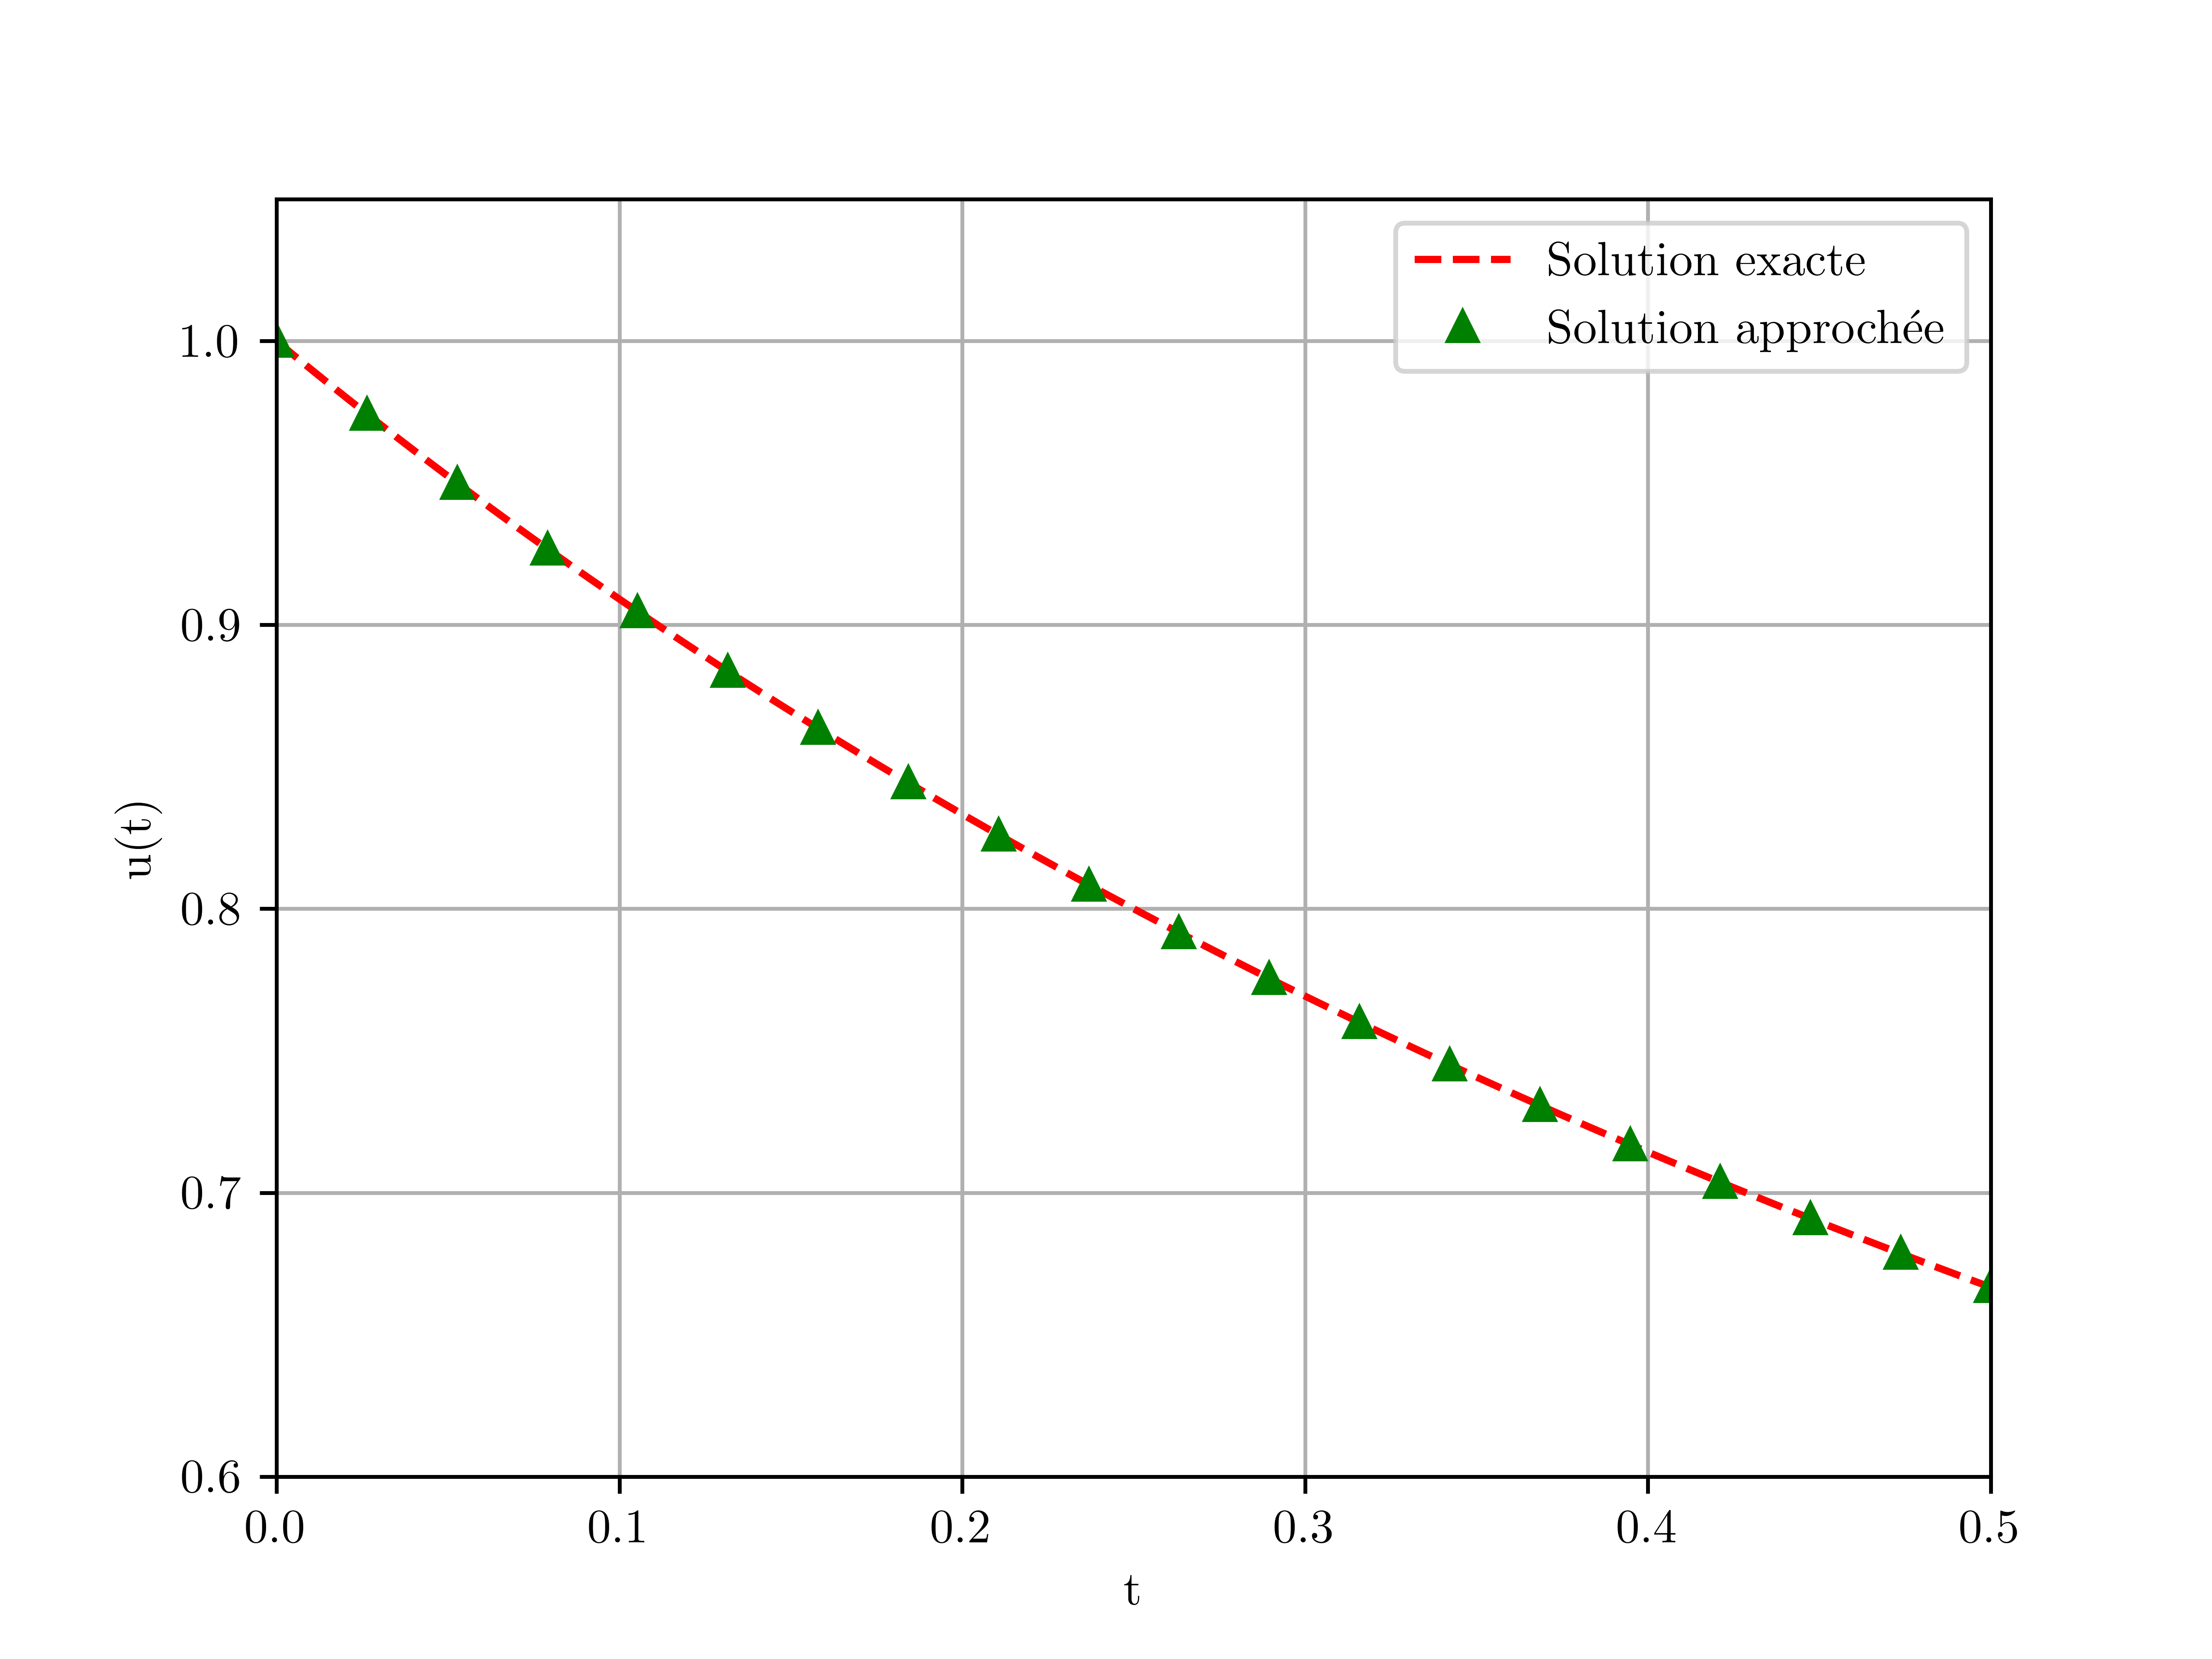
\includegraphics[scale = 0.7]{IMAGES/plot.png}
    \caption{Comparaison entre la solution exacte et la solution approchée en utilisant la MPH.}
    \label{fig:sol_EDO_1}
\end{figure}
\subsubsection*{Exemple 2}
Maintenant, nous allons considérer l'équation de Lane-Emden suivante:
\begin{equation}\label{ex:EDO_2}
    \begin{cases}
        u''(x)+\frac{2}{x}u'(x)+u(x) = x^5 + 30x^3,\\
        u(0) = u'(0)=0,
    \end{cases}
\end{equation}
où la solution exacte est exprimée par:
\begin{equation}
    u(x)=x^5.
\end{equation}
La méthode de perturbation d'Homotopie, implique :
\begin{equation} \label{sol:EDO_2}
    \left(v''+\frac{2}{x}v'\right) - \left(u''_0+\frac{2}{x}u'_0 \right) = p\left(x^5+30x^3-v-u''_0 - \frac{2}{x}u'_0\right).
\end{equation}
La solution de l'équation \ref{ex:EDO_2} est sous la forme:
\begin{equation}
    v=v_0+pv_1+p^2v_2+p^3v_3 + ...
\end{equation}
Substituons l'équation \ref{sol:EDO_2} dans l'équation \ref{ex:EDO_2} et identifions les termes de même puissance de $p$, il vient :\\
\begin{align*}
    \begin{cases}
        &p^0 : v_0(x) = u_0(x)=0,\\
        &p^1 : v_1(x)=\frac{1}{56}x^7 + x^5,\\
        &p^2 : v_2(x) = -\frac{1}{5040}x^9 - \frac{1}{56}x^7,\\
        &p^3 : v_3(x) = \frac{1}{665280}x^{11}+\frac{1}{5040}x^9,\\
        &p^4 : v_4(x) = \frac{1}{121080960} x^{13} - \frac{1}{665280}x^{11},\\
        &p^5 : v_5(t) = \frac{1}{29059430400}x^{15} + \frac{1}{121080960} x^{13},\\
        &    .\\
        &    .\\
        &    .\\
    \end{cases}
\end{align*}
Finalement, la solution approchée le d'équation \ref{ex:EDO_2} est donnée par:
\begin{equation}
    u(x)=\lim_{p\to 1} v(x)=v_0(x)+v_1(x)+v_2(x)+...
\end{equation}
\begin{figure}[H]
    \centering
    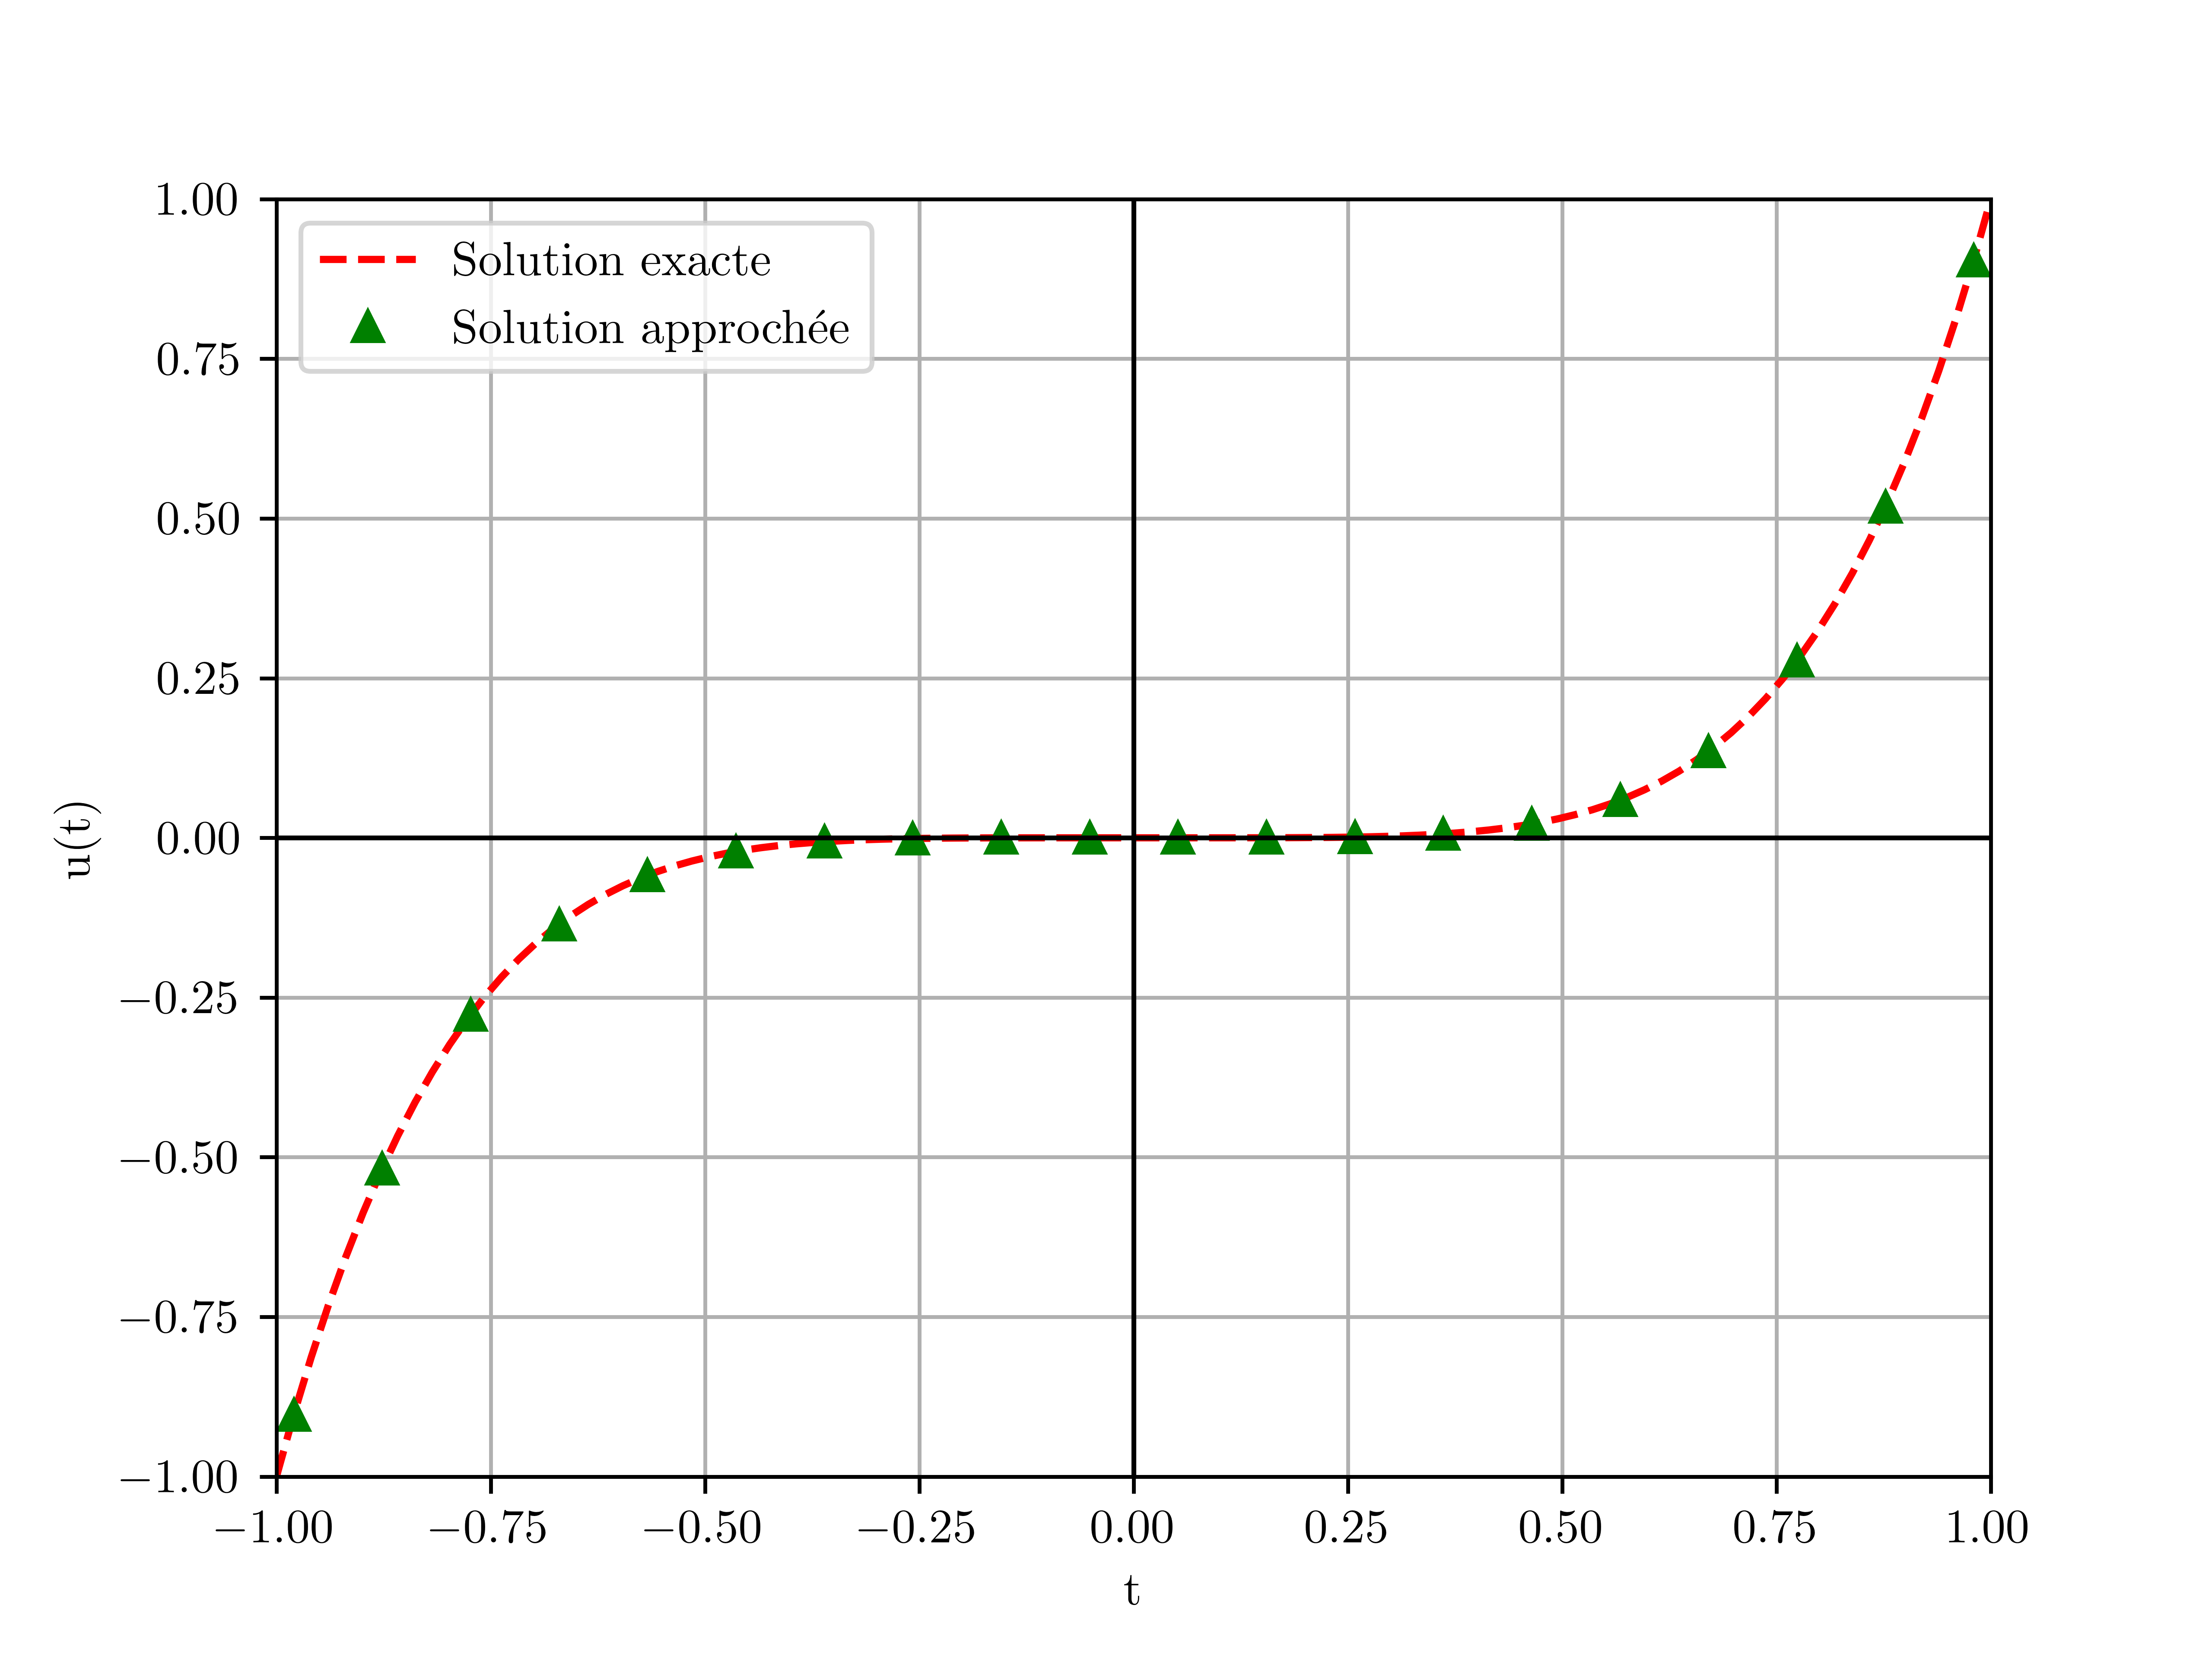
\includegraphics[scale = 0.7]{IMAGES/plot (2).png}
    \caption{Comparaison entre la solution exacte et la solution approchée en utilisant la MPH.}
\end{figure}



\section{Application de la méthode aux équations différentielles fractionnaires}
\subsection{Description de la méthode}
 Le problème de valeur initiale d'équations différentielles fractionnaires est donnée par sa forme opérationnelle:
 \begin{align}\label{eq: HMP_EDF_theorie}
     D^{\alpha} f(t) + Lf(t) = g(t)\\
     f^{(i)} (0) = c_i, \hspace{1cm} i=0,1,2, ..., n-1
 \end{align}
 où $c_i$ est la condition initial, $L$ désigne un opérateur linéaire qui peut inclus d'autre opérateurs de dérivées fractionnaires $D^{\beta}(\beta < \alpha)$ et $g$ est une fonction connue.
\\
L'homotopie de l'équation \ref{eq: HMP_EDF_theorie} satisfait :
  \begin{equation}\label{eq:HPM_FDE_1}
      (1-p)D^{\alpha} f +p\left[ D^{\alpha}f + Lf(t) -g(t)\right]=0, \hspace{1cm} p\in [0,1],
  \end{equation}
  où
  \begin{equation}\label{eq:HPM_FDE_2}
      D^{\alpha}f+p\left[Lf(t)-g(t)\right]=0,
  \end{equation}
  avec $p\in[0,1]$ est un paramètre d'homotopie. Si $p=0$, l'équation \ref{eq:HPM_FDE_1} et \ref{eq:HPM_FDE_2} devient:
  \begin{equation}
      D^{\alpha} f=0
  \end{equation}
  Si $p=1$, les deux équations \ref{eq:HPM_FDE_1} et \ref{eq:HPM_FDE_2} donnent l'EDF original \ref{eq: HMP_EDF_theorie}.\\
  La solution de l'équation \ref{eq: HMP_EDF_theorie} est:
  \begin{equation} \label{eq:sol_HPM_theorie}
      f(t)=f_0(t)+pf_1(t)+p^2f_2(t)+p^3f_3(t) + ...
  \end{equation}
  Substituons l'équation \ref{eq:sol_HPM_theorie} dans l'équation \ref{eq:HPM_FDE_2} et identifions les termes de même puissance de $p$, il vient:
  \begin{align*}
  \begin{cases}
            & p^0 : D^{\alpha} f_0 = 0\\
      & p^1 : D^{\alpha} f_1 = -Lf_0 + g(t)\\
      & p^2 : D^{\alpha} f_2 = -Lf_1(t)\\
      & p^3 : D^{\alpha} f_3 = -Lf_2(t)\\
      & .\\
      & .\\
  \end{cases}
  \end{align*}
on peut réécrit les termes de solution de perturbation d'homotopie par :
\begin{align*}
    \begin{cases}
        & f_0 = \sum_{i=O}^{m-1} f^{(i)}(0) \frac{t^i}{i!} = \sum _{i=0}^{m-1} c_i \frac{t^i}{i!} \\
          & f_1 = -I^{\alpha} [Lf_0(t)] + I^{\alpha}[Lg(t)]\\
          & f_2 = -I^{\alpha}[Lf_1(t)]\\
          & f_3 = -I^{\alpha}[Lf_2(t)]\\
          & .\\
          & .\\
    \end{cases}
  \end{align*}
La forme générale de la solution HPM est donné par :
\begin{equation}
    f_n=-I^{\alpha}[Lf_{n-1}(t)]
\end{equation}
Alors la solution de perturbation d'homotopie est :
\begin{equation}
    f(t)=f_0+f_1+f_2+f_3 + ... +f_n + ...
\end{equation}
\subsection{Application}
\subsubsection*{Exemple 1}
Considérons l'équation différentielle fractionnaire linéaire suivante:
\begin{equation}
    \begin{cases}\label{ex:EDF_1}
        D^{\alpha}x(t) + x(t) = \frac{2}{\Gamma(3-\alpha)} t^{2-\alpha} + t^3,\\
        x(0)=0,\\
        x'(0)=0.
    \end{cases}
\end{equation}
où la solution exacte pour $\alpha = 1,9$ est donnée par:
\begin{equation}
    x(t)=t^2.
\end{equation}
Selon la méthode de perturbation d'Homotopie, nous pouvons construire l'homotopie suivante:
\begin{equation} \label{eq:HPM_EDF1}
    D^{\alpha} x(t) +p\left[x(t)-\frac{2}{\Gamma(3-\alpha)}t^{2-\alpha}-t^3\right] =0, \hspace{1cm} t\in \Omega,
\end{equation}
La solution de \ref{ex:EDF_1} peut être exprimée comme suit :
\begin{equation}\label{sol:EDF_1}
    x(t) =x_0(t) + px_1(t) + p^2x_2(t) + ... = \sum _{i=O}^{\infty} p^i x_i(t)
\end{equation}
Substituons l'équation \ref{sol:EDF_1} dans l'équation \ref{eq:HPM_EDF1} et identifions les termes de même puissance de $p$, il vient :
\begin{align*}
    \sum_{i=0}^{\infty} D^{\alpha} p^{(i)} x_i(t) = -p\left[\sum_{i=0}^{\infty} p^{(i)} x_i(t) -\frac{2}{\Gamma(3-\alpha)} t^{2-\alpha} -t^3\right]
\end{align*}
\begin{align} \label{eq:p_1}
    \begin{cases}
    & p^0 : D^{\alpha}x_0(t)=0, \\
    & p^1 : D^{\alpha}x_1(t) = -x_0(t) + \frac{2}{\Gamma(3-\alpha)} t^{2-\alpha} + t^3,\\
    & p^2 : D^{\alpha} x_2(t) = -x_1(t),\\
    & p^3 : D^{\alpha} x_3(t) = -x_2(t),\\
    &     . \\
    &     .\\
    &     .\\
    \end{cases}
\end{align}
Appliquent l'opérateur $I^{\alpha}$ sur les deux cotés de d'équations \ref{eq:p_1} et on utilisons les propriétés de L'intégrale fractionnaire de Riemann-Liouville d'ordre $\alpha \geq 0$, on obtient 
\begin{align*}
    I^\alpha D^{\alpha} x_0(t) &= x_0(t)-\sum_{i=0}^1 \frac{x^{(i)}(0) t^i}{i!},\\
    &= x_0(t)-x(0)\frac{t^0}{0!}-x'(0)\frac{t^1}{1!}\\
    &= x_0(t) = 0
\end{align*}
\begin{align*}
    I^{\alpha}D^{\alpha}x_1(t)&=x_1(t)-\sum_{i=0}^1 \frac{x^{(i)}(0) t^i}{i!} = x_1(t)\\
    x_1(t) &= I^{\alpha} \left[-x_0(t)+\frac{2}{\Gamma(3-\alpha)}t^{2-\alpha}+t^3\right]\\
    & = I^{\alpha} \left[\frac{2}{\Gamma(3-\alpha)}t^{2-\alpha}+t^3\right]\\
    & = I^{\alpha} \left[\frac{2}{\Gamma(3-\alpha)}t^{2-\alpha}\right]+I^{\alpha}\left[t^3\right]\\
    &= \left[\frac{2}{\Gamma(3-\alpha)} \frac{\Gamma(3-\alpha)}{\Gamma(3-\alpha + \alpha)}t^{\alpha+2-\alpha}\right] + \left[\frac{\Gamma(4)}{\Gamma(4+\alpha)}t^{\alpha+3} \right]\\
    &= \frac{2}{(3-1)!} t^2 + \frac{\Gamma(4)}{\Gamma(4+\alpha)} t^{\alpha +3}\\
    &= t^2 + \frac{\Gamma(4)}{\Gamma(4+\alpha)}t^{\alpha+3}
\end{align*}
\begin{align*}
    I^{\alpha}D^{\alpha}x_2(t)&=x_2(t)-\sum_{i=0}^1 \frac{x^{(i)}(0) t^i}{i!} = x_2(t)\\
    x_2(t) &= -I^{\alpha}[x_1(t)]\\
    &= -I^{\alpha} \left[t^2 + \frac{\Gamma(4)}{\Gamma(4+\alpha)}t^{3+\alpha} \right]\\
    &= -I^{\alpha}\left[t^2\right] -I^{\alpha} \left[\frac{\Gamma(4)}{\Gamma(4+\alpha)}t^{3+\alpha} \right]\\
    &= -\frac{\Gamma(3)}{\Gamma(3+\alpha)}t^{\alpha+2} - \frac{\Gamma(4)}{\Gamma(4+\alpha)}\frac{\Gamma(4+\alpha)}{\Gamma(4+2\alpha)}t^{3+2\alpha}\\
    &= -\frac{2}{\Gamma(3+\alpha)} t^{\alpha+2} - \frac{6}{\Gamma(4+2\alpha)}t^{3+2\alpha}\\
\end{align*}
\begin{align*}
    I^{\alpha}D^{\alpha}x_3(t) &= x_3(t) - \sum_{i=0}^{1} \frac{x^{(i)}(0)t^i}{i!} = x_3(t)\\
    x_3(t) &= -I^{\alpha} [x_3(t)]\\
    &= -I^{\alpha} \left[ -\frac{2}{\Gamma(3+\alpha)} t^{\alpha+2} - \frac{6}{\Gamma(4+2\alpha)}t^{3+2\alpha}\right]\\
    &= -I^{\alpha} \left[ -\frac{2}{\Gamma(3+\alpha)} t^{\alpha+2} \right] - I^{\alpha} \left[ - \frac{6}{\Gamma(4+2\alpha)}t^{3+2\alpha} \right]\\
    &= \frac{2}{\Gamma(3+\alpha)}\frac{\Gamma(3+\alpha)}{\Gamma(3+2\alpha)} t^{2+2\alpha} + \frac{6}{\Gamma(4+2\alpha)} \frac{\Gamma(4+2\alpha)}{\Gamma(3+3\alpha)}t^{3+3\alpha}\\
    &= \frac{2}{\Gamma(3+2\alpha)}t^{2+2\alpha} + \frac{6}{\Gamma(3+3\alpha)} t^{3+3\alpha}.
\end{align*}
Nous obtenons:
\begin{align*}
    &x _0(t)=0\\
    & x_1(t) = \frac{2}{\Gamma(3-\alpha)}t^{2-\alpha} + t^3\\
    & x_2(t) = -\frac{2}{\Gamma(3-\alpha)} t^{2-\alpha} -t^3\\
    & x_3(t) = \frac{2}{\Gamma(3+2\alpha)}t^{2+2\alpha} + \frac{6}{\Gamma(3+3\alpha)} t^{3+3\alpha} \\
    & .\\
    & .\\
\end{align*}
Donc la solution de l'équation \ref{ex:EDF_1} est donnée par:
\begin{align*}
        x(t) &= x_0(t) + px_1(t) + p^2x_2(t) + p^3x_3(t)+...\\
        & = 0 + t^2 + \frac{\Gamma(4)}{\Gamma(4+\alpha)} -\frac{2}{\Gamma(3+\alpha)} t^{2+\alpha} -\frac{6}{\Gamma(4+2\alpha)} t^{3+2\alpha} + \frac{2}{\Gamma(3+2\alpha)}t^{2+2\alpha} +...
\end{align*}
si $\alpha = 1,9$
\begin{align*}
    x(t) &= t^2 + \frac{6}{\Gamma(5,9)}t^{4,9} -\frac{2}{4,9)}t^{3,9} - \frac{6}{\Gamma(7,8)}t^{6,8} + ...\\
    &= t^2 + 0.059247439t^{4,9} - 0.096770806t^{3,9} - 0.001776766299 t^{6,8} + ...\\
    & \approx t^2
\end{align*}
En utilisant les solutions exactes trouvées dans l'article \cite{Numerical_sol}, et en calculant les solutions approchées à l'aide de la méthode de perturbation d'homotopie avec Wolfram Alpha, voici le tableau \ref{tab:1} qui affiche les valeurs numériques des solutions exactes, solutions approchées ainsi que l'erreur entre les deux solutions. De plus, la figure suivante compare les deux résultats. 
\begin{figure}[H]
    \centering
    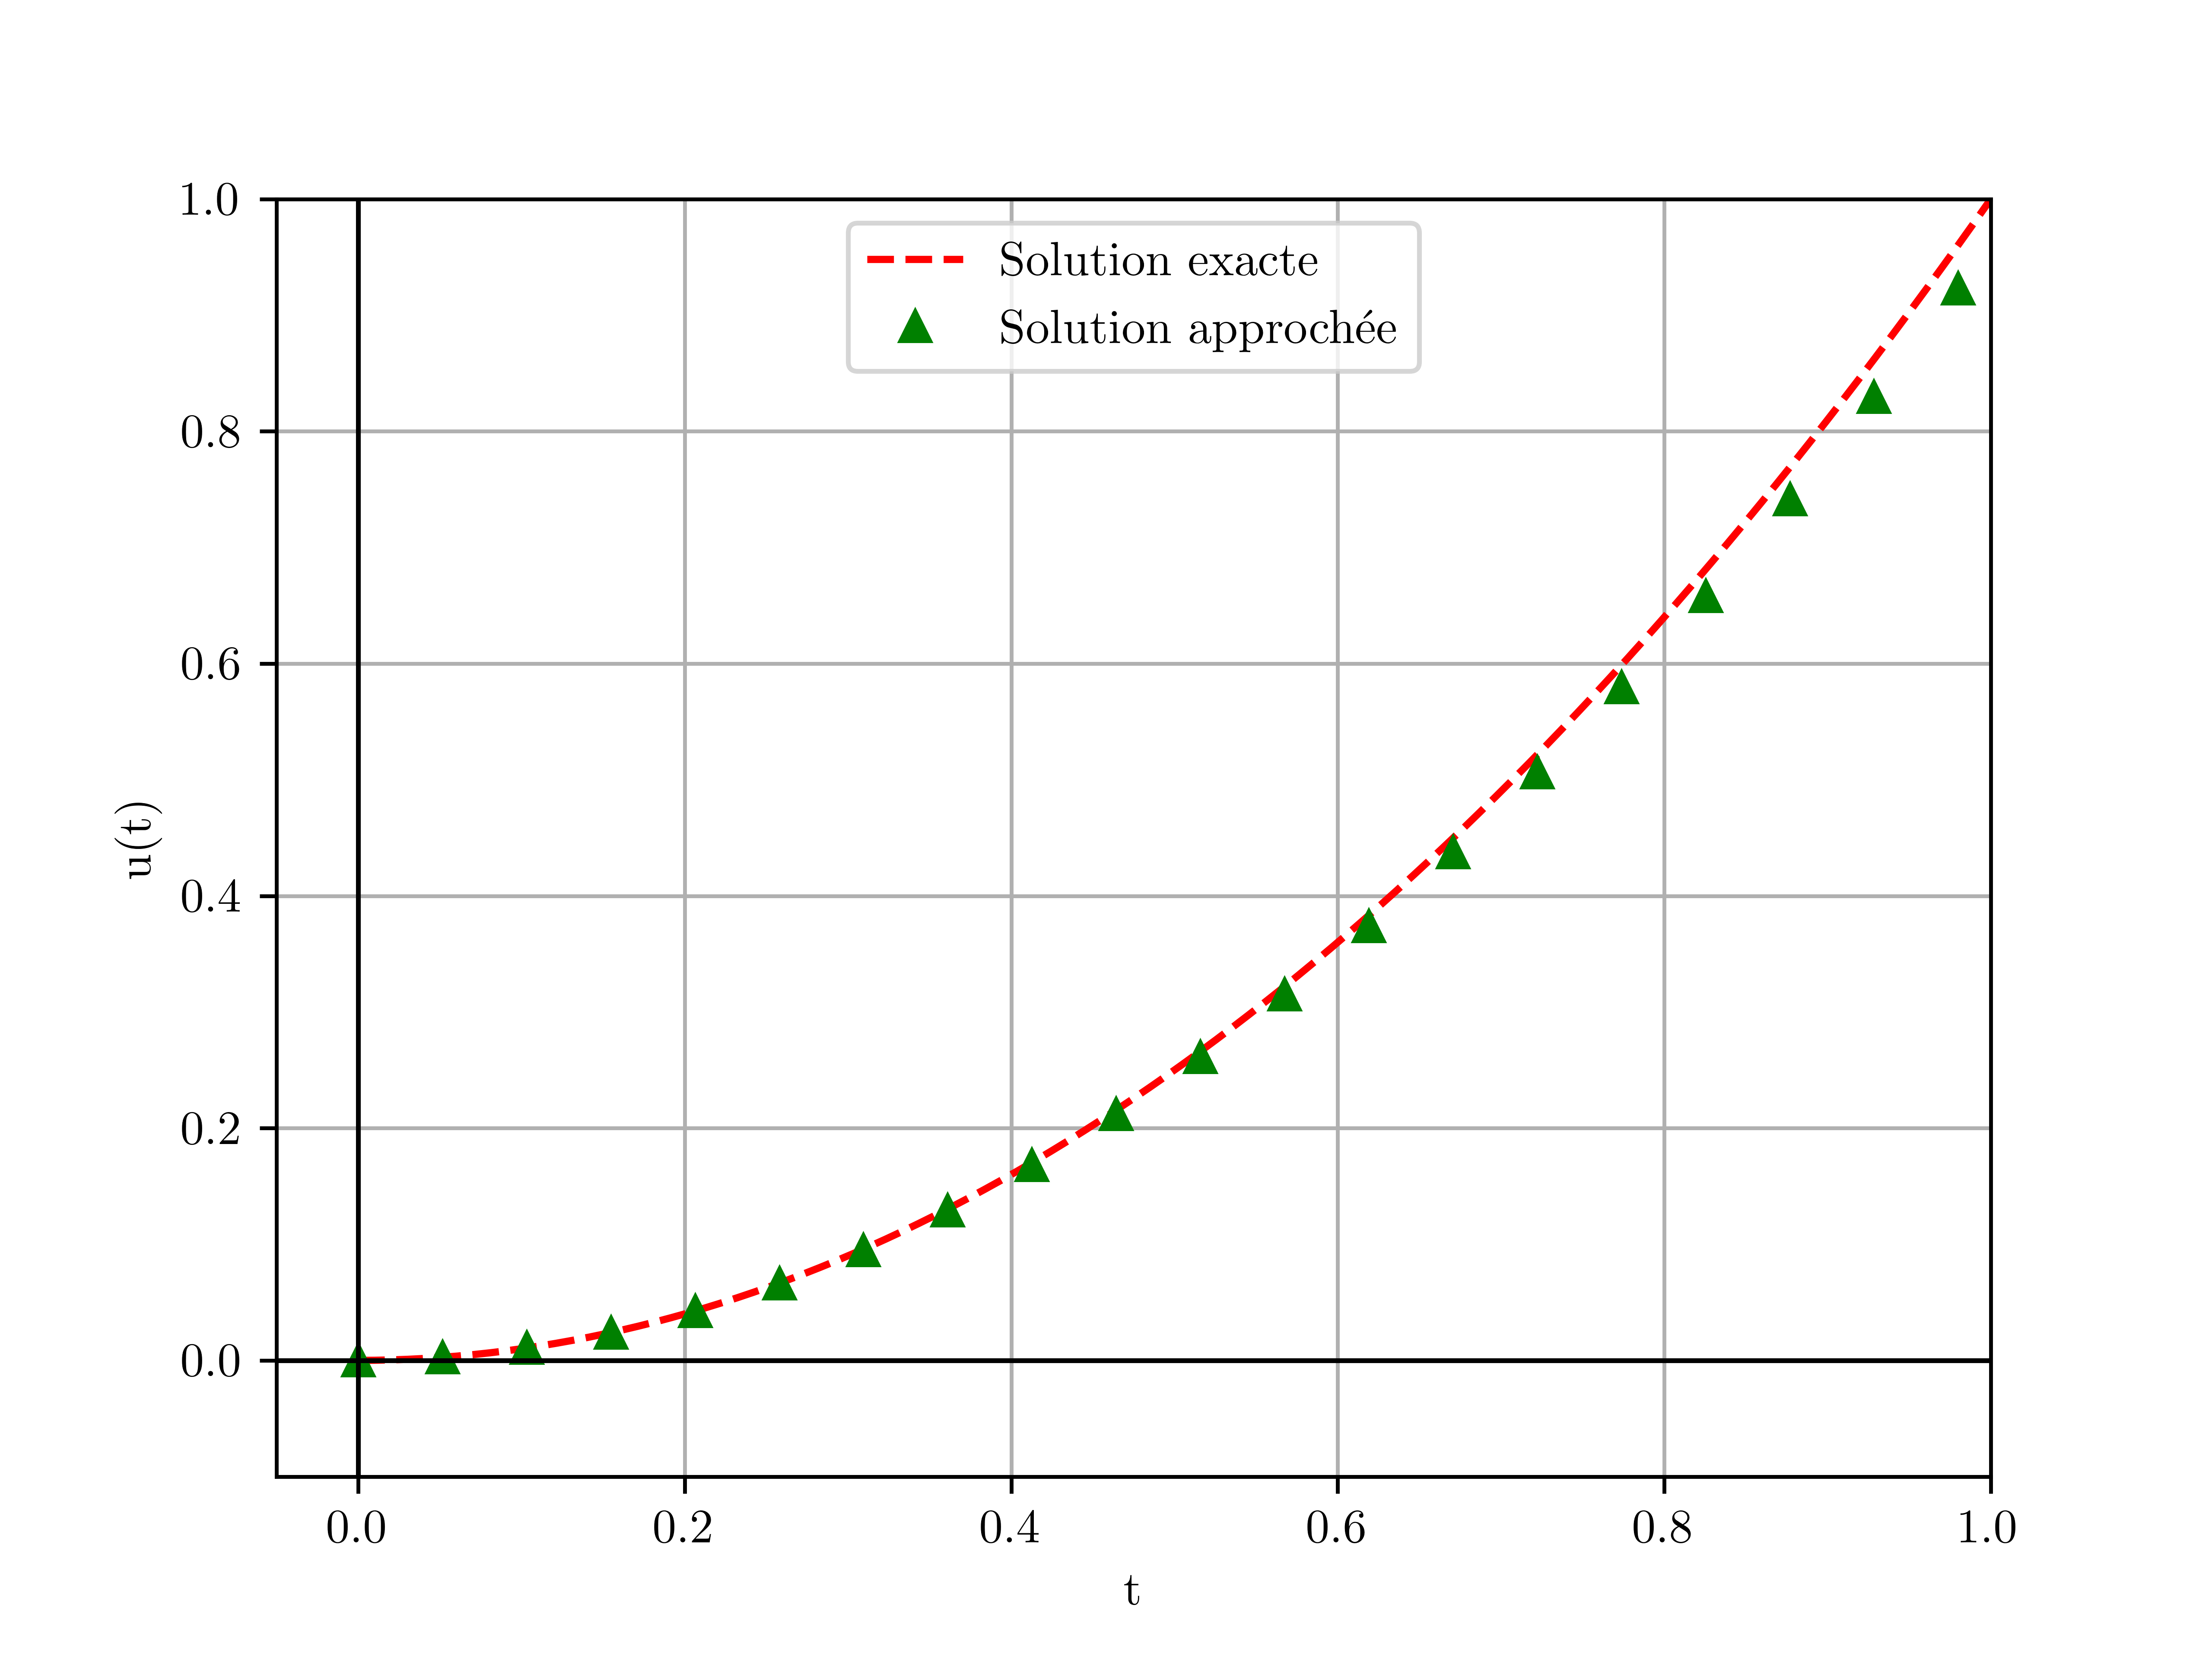
\includegraphics[scale = 0.7]{IMAGES/plot (3).png}
    \caption{Comparaison entre la solution exacte et la solution approchée en utilisant la MPH.}
\end{figure}

\subsubsection*{Exemple 2}
Maintenant, considérons la deuxième équation différentielle factionnaire linéaire suivante :
\begin{equation}\label{ex:EDF_2}
    \begin{cases}
        D^{\alpha} x(t) +x(t) = 1\\
        x(0)=0\\
        x'(t) =0
    \end{cases}
\end{equation}
où la solution exacte est donnée par:
\begin{equation}
    x(t)=t^{1,1} E_{1,1. 2,1} (-t^{1,1})
\end{equation}
Selon la méthode de perturbation d'Homotopie, nous pouvons construire l'homotopie suivante:
\begin{equation} \label{eq:HPM_EDF2}
    D_{\alpha} x(t) +p\left[x(t)-1\right]=0
\end{equation}
La solution de \ref{ex:EDF_1} peut être exprimée comme suit :
\begin{equation}\label{sol:EDF_2}
    x=x_0 + px_1 + p^2x_2 ... = \sum _{i=0}^{\infty} p^i x_i
\end{equation}
Substituons l'équation \ref{sol:EDF_2} dans l'équation \ref{eq:HPM_EDF2} et identifions les termes de même puissance de $p$, il vient :
\begin{align*}
    \sum_{i=0}^{\infty} D^{\alpha} p^{(i)}x_i(t) = p\left(1-\sum_{i=0}^{\infty} p^{i}x_i (t) \right)
\end{align*}
\begin{align}\label{eq:p_2}
\begin{cases}
    & p^0 : D^{\alpha}x_0(t)=0, \\
    & p^1 : D^{\alpha}x_1(t) = 1 -x_0(t),\\
    & p^2 : D^{\alpha} x_2(t) = -x_1(t),\\
    & p^3 : D^{\alpha} x_3(t) = -x_2(t),\\
    &     . \\
    &     .\\
    &     .\\
\end{cases}
\end{align}
Appliquent l'opérateur $I^{\alpha}$ sur les deux cotés de d'équations \ref{eq:p_2} et on utilisons les propriétés de L'intégrale fractionnaire de Riemann-Liouville d'ordre $\alpha \geq 0$, on obtient \begin{align*}
    I^\alpha D^{\alpha} x_0(t) &= x_0(t)-\sum_{i=0}^1 \frac{x^{(i)}(0) t^i}{i!},\\
    &= x_0(t)-x(0)\frac{t^0}{0!}-x'(0)\frac{t^1}{1!}\\
    &= x_0(t) = 0
\end{align*}
\begin{align*}
    I^{\alpha} D^{\alpha}x_1(t) &= x_1(t) - \sum_{i=0}^1 \frac{x^{(i)}(0) t^i}{i!} = x_1(t)\\
    x_1(t) &= I^{\alpha} \left[1-x_0(t)\right]\\
    &= I^{\alpha} [1]\\
    &= \frac{t^{\alpha}}{\Gamma(\alpha +1)}.
\end{align*}
\begin{align*}
    I^{\alpha} D^{\alpha}x_2(t) &= x_2(t) - \sum_{i=0}^1 \frac{x^{(i)}(0) t^i}{i!} = x_2(t)\\
    x_2(t) &= - I^{\alpha} \left[\frac{t^{\alpha}}{\Gamma(\alpha +1)}\right]\\
    &= -\frac{1}{\Gamma(\alpha +1)} \frac{\Gamma(\alpha+1)}{\Gamma(2\alpha +1)} t^{2\alpha}\\
    & = - \frac{t^{2\alpha}}{\Gamma(2\alpha+1)}.
\end{align*}
\begin{align*}
     I^{\alpha} D^{\alpha}x_3(t) &= x_3(t) - \sum_{i=0}^1 \frac{x^{(i)}(0) t^i}{i!} = x_3(t)\\
    x_3(t) &= - I^{\alpha} \left[ - \frac{t^{2\alpha}}{\Gamma(2\alpha+1)} \right]\\
    &= \frac{1}{\Gamma(2\alpha +1)} \frac{\Gamma(2\alpha+1)}{\Gamma(2\alpha +1 + \alpha)} t^{2\alpha + \alpha}\\
    & = \frac{t^{3\alpha}}{\Gamma(3\alpha+1)}.
\end{align*}
Nous obtenons :
\begin{align*}
    & x_0(t) = 0\\
    & x_1(t) = \frac{t^{\alpha}}{\Gamma(\alpha +1)}\\
    & x_2(t) = -\frac{t^{2\alpha}}{\Gamma(2\alpha +1)}\\
    & x_3(t) = \frac{t^{3\alpha}}{\Gamma(3\alpha+1)}\\
    & . \\
    & . \\
\end{align*}
Donc la solution de l'équation \ref{ex:EDF_2} est donnée par:
\begin{align*}
        x(t) &= x_0(t) + px_1(t) + p^2x_2(t) + p^3x_3(t)+...\\
        & = 0 + \frac{t^{\alpha}}{\Gamma(\alpha +1)} -\frac{t^{2\alpha}}{\Gamma(2\alpha +1)} + \frac{t^{3\alpha}}{\Gamma(3\alpha+1)} +...\\
        &= \sum_{K=1}^{\infty}(-1)^{k+1}\frac{t^{k\alpha}}{\Gamma(k\alpha +1)}
\end{align*}
si $\alpha = 1,1$
\begin{align*}
    x(t) &= \frac{t^{1,1}}{\Gamma(2,1)} - \frac{t^{2,2}}{\Gamma(3,2)} +\frac{t^{3,3}}{\Gamma(4,3)} - \frac{t^{4,4}}{\Gamma(5,4)}+...\\
    &= \frac{t^{1,1}}{0.95135} - \frac{t^{2,2}}{0,95135} +\frac{t^{3,3}}{0.95135} - \frac{t^{4,4}}{0.95135}+...\\
    & = 0.95557t^{1,1} - 0.41255t^{2,2} + 0.11293t^{3,3}- 0.02242 t^{4,4} + ...
\end{align*}
De même, en utilisant les solutions exactes extraites de l'article \cite{Numerical_sol} et en déterminant les solutions approchées grâce à la méthode de perturbation d'homotopie, calculées à l'aide de Wolfram Alpha., nous obtenons le tableau \ref{tab:2}. Ce tableau présente les valeurs numériques des solutions exactes, des solutions approchées, ainsi que l'erreur entre ces deux types de solutions. En outre, une comparaison des deux résultats est illustrée dans la figure ci-dessous.
\begin{figure}[H]
    \centering
    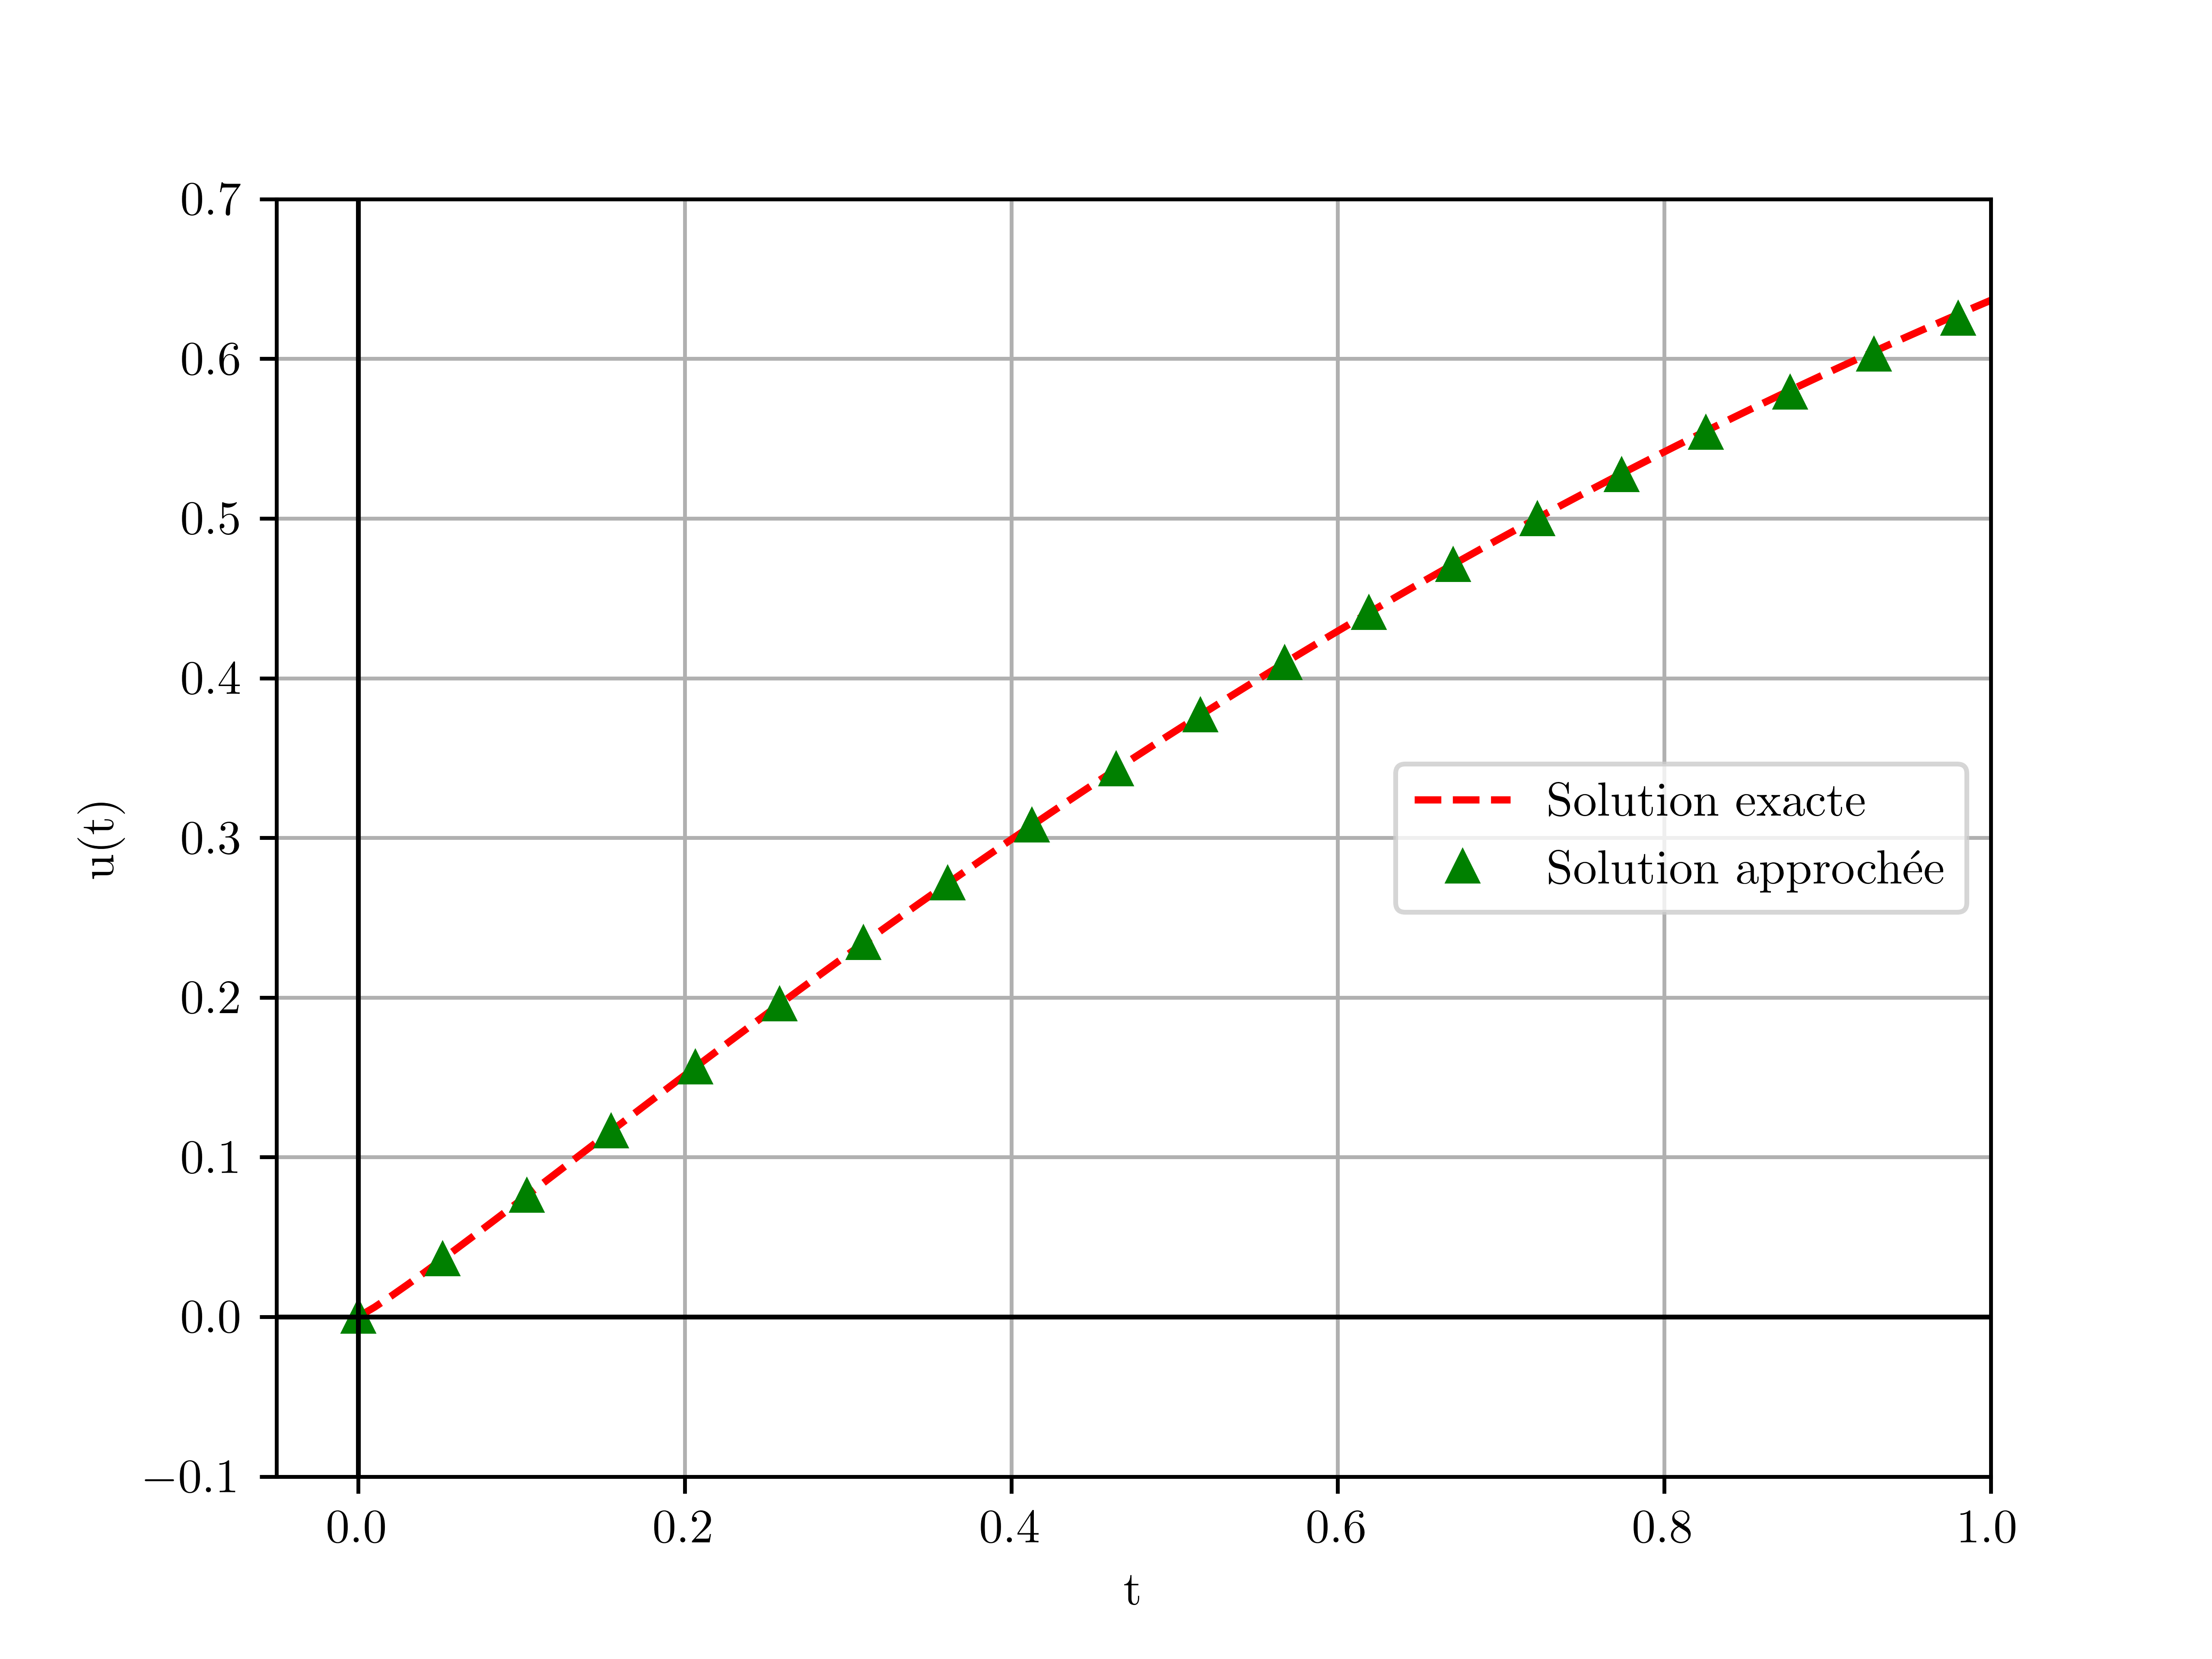
\includegraphics[scale = 0.7]{IMAGES/plot (6).png}
    \caption{Comparaison entre la solution exacte et la solution approchée en utilisant la MPH.}
\end{figure}

% CONCLUSIONS

%%%%%%%%%%%%%%%%%%%%%%%%%%%%%%%%%%%%%%%%%%%%%%%%%%
%%%%		~~~~ Conclusion ~~~~
%%%%%%%%%%%%%%%%%%%%%%%%%%%%%%%%%%%%%%%%%%%%%%%%%%


\chapter{Conclusion générale}
\label{chap:Conclusion}
\pagestyle{fancy}

En conclusion, ce travail a présenté une étude détaillée sur une des méthodes numériques pour résoudre les EDF, la perturbation d'homotopie. Nous avons commencé par discuter les fondamentaux mathématiques et expliquer en profondeur les dérivées et intégrales fractionnaires.

Nos résultats numériques, qui comparent les solutions exactes et approximatives, démontrent une précision remarquable et satisfaisante de la méthode de perturbation d'homotopie. En effet, les erreurs calculées sont de l'ordre de 10$^{-6}$, ce qui indique une haute précision des solutions approximatives par rapport aux solutions exactes.

Il convient de souligner l'importance des outils computationnels dans notre étude. Nous avons utilisé Python pour générer les figures des fonctions spéciales et comparer les solutions, tandis que Wolfram Alpha a été d'une aide précieuse pour calculer efficacement nos solutions approximatives. Cela illustre l'importance d'une approche interdisciplinaire combinant mathématiques et informatique dans le domaine de la résolution numérique des EDFs.

Cependant, bien que la méthode de perturbation d'homotopie soit efficace et intuitive, elle est l'une parmi plusieurs approches pour résoudre les EDFs. D'autres méthodes pourraient offrir de meilleurs résultats.






% SETTING FOR APPENDIX ENVIRONMENT
{
\noappendicestocpagenum
\renewcommand{\appendixtocname}{Annexes}
\renewcommand{\appendixpagename}{Annexes}
\appendix
\addappheadtotoc
\normalsize
}
\appendix

% APPENDIX
%%%%%%%%%%%%%%%%%%%%%%%%%%%%%%%%%%%%%%%%%%%%%%%%%%
%%%%		~~~~ Appendix example ~~~~
%%%%%%%%%%%%%%%%%%%%%%%%%%%%%%%%%%%%%%%%%%%%%%%%%%

\chapter{Code python}
% START APPENDIX
\section{Visualisation des fonctions}

\lstset{
  language=Python,
  showspaces=false,
  showstringspaces=false,
  breaklines=true,
  postbreak=\raisebox{0ex}[0ex][0ex]{\ensuremath{\color{red}\hookrightarrow\space}},
  basicstyle=\ttfamily,
}

\subsubsection*{La fonction Gamma}

\noindent
\begin{minted}[mathescape,
               linenos,
               numbersep=5pt,
               gobble=2,
               frame=lines,
               framesep=2mm,
               fontsize=\footnotesize]{Python}
    import numpy as np
    import matplotlib.pyplot as plt
    from scipy.special import gamma
    
    # plot gamma function
    x = np.linspace(0.0001, 5, 200)
    y = gamma(x)
    
    plt.plot(x, y, 'r--', label="Gamma function")
    plt.grid()
    plt.xlim(-.05, 5)
    plt.ylim(-.1, 20)
    plt.xlabel(r"x")
    plt.ylabel(r"$\Gamma(x)$")
    plt.legend()
    plt.show()
\end{minted}
\subsubsection*{La relation entre la fonction Gamma et la Factorielle
}

\noindent
\begin{minted}[mathescape,
               linenos,
               numbersep=5pt,
               gobble=2,
               frame=lines,
               framesep=2mm,
               fontsize=\footnotesize]{Python}
    import numpy as np
    from scipy.special import gamma, factorial
    import matplotlib.pyplot as plt
    
    x = np.linspace(-3.5, 5.5, 2251)
    y = gamma(x)
    
    plt.plot(x, y, 'b', alpha=0.6, label='gamma(x)')
    
    k = np.arange(1, 7)
    
    plt.plot(k, factorial(k-1), 'k*', alpha=0.6, label='(x-1)!, x = 1, 2, ...')
    
    plt.xlim(-3.5, 5.5)
    plt.ylim(-10, 25)
    plt.grid()
    plt.xlabel('x')
    plt.legend(loc='lower right')
    
    plt.show()
\end{minted}
D'après la documentation de scipy \cite{plot:wiki_gamma}

\subsubsection*{La fonction Bêta}

\noindent
\begin{minted}[mathescape,
               linenos,
               numbersep=5pt,
               gobble=2,
               frame=lines,
               framesep=2mm,
               fontsize=\footnotesize]{Python}
    from mpl_toolkits.mplot3d import axes3d
    import matplotlib.pyplot as plt
    import numpy as np
    from scipy.special import beta
    
    # Prepare the data by Beta(x, y)
    X = np.arange(0.03, 4.0, .01)
    Y = np.arange(0.03, 4.0, .01)
    Z = np.ndarray(shape=(len(X), len(Y)), dtype = float)
    for i in range(len(X)):
            for j in range(len(Y)):
                    Z[i][j] = beta(X[i], Y[j])
    # Draw the data
    fig = plt.figure()
    ax = fig.add_subplot(111, projection='3d')
    gridX, gridY = np.meshgrid(X, Y)
    ax.plot_surface(gridX, gridY, Z, lw=0.0, cmap='Reds')
    # ax.azim = 180
    ax.elev = 30
    plt.xticks([0, 1, 2, 3, 4])
    plt.yticks([0, 1, 2, 3, 4])
    ax.contour(X, Y, Z, zdir='z', offset=0, cmap='Greens')
    ax.set_xlim([4.0, 0.0])
    ax.set_ylim([4.0, 0.0])
    ax.set_zlim([0, 50])
    ax.set_xlabel(r'$x$')
    ax.set_ylabel(r'$y$')
    ax.set_zlabel(r'$\beta(x, y)$')
    # fig.savefig('betaFunc.png', transparent=True, dpi=800)
    plt.show()
\end{minted}
D'après "Wikimedia Commens" (modifié) \cite{plot:wiki_beta}

\subsubsection*{La fonction Mittag-Leffler}

\noindent
\begin{minted}[mathescape,
               linenos,
               numbersep=5pt,
               gobble=2,
               frame=lines,
               framesep=2mm,
               fontsize=\footnotesize]{Python}
    import numpy as np
    
    def mittag_leffler(alpha, beta, t, terms=100):
    k = np.asarray([((t**k) / gamma(alpha * k + beta)) for k in range(terms)])
    return k.sum(0)
\end{minted}

\section{Visualisation des solutions exactes et approximatives}
\subsubsection*{Exemple : \ref{ex:EDO_1}}

\noindent
\begin{minted}[mathescape,
               linenos,
               numbersep=5pt,
               gobble=2,
               frame=lines,
               framesep=2mm,
               fontsize=\footnotesize]{Python}
    import numpy as np
    import matplotlib.pyplot as plt
    import matplotlib
    # use latex
    plt.rcParams.update({
        "text.usetex": True,
        "font.family": "Computer Modern"
    })
    
    # Functions
    x = np.linspace(0, 0.5, 100)
    x_2 = np.linspace(0, 0.5, 20)
    y = 1 / (1 + x)
    y_2 = 1 - x_2 + x_2**2 - x_2**3 + x_2**4 - x_2**5 + x_2**6 - x_2**7 + x_2**8 - x_2**9 
    + x_2**10
    
    plt.plot(x, y, 'r--', label="Solution exacte")
    plt.plot(x_2, y_2, 'g^', label="Solution approchée")
    plt.grid()
    plt.xlim(0, 0.5)
    plt.ylim(0.6, 1.05)
    plt.xlabel("t")
    plt.ylabel("u(t)")
    plt.legend()
    plt.savefig("plot.png", transparent=True, dpi=800)
\end{minted}
\subsubsection*{Exemple : \ref{ex:EDO_2}}

\noindent
\begin{minted}[mathescape,
               linenos,
               numbersep=5pt,
               gobble=2,
               frame=lines,
               framesep=2mm,
               fontsize=\footnotesize]{Python}
    import numpy as np
    2 from scipy.special import gamma, factorial
    3 import matplotlib.pyplot as plt
    
    x = np.linspace(-1, 1, 100)
    x_2 = np.linspace(-0.98, 0.98, 20)
    y = x  5
    y_2 = (x_2**5 + ((1/56) * x_2**7)) - ((1/5040) * (x_2**9) + (1/56) * (x_2  7))
    
    plt.plot(x, y, 'r--', label="Solution exacte")
    plt.plot(x_2, y_2, 'g^', label="Solution approchée")
    plt.grid()
    plt.xlim(-1, 1)
    plt.ylim(-1, 1)
    plt.xlabel("t")
    plt.ylabel("u(t)")
    plt.legend()
    plt.axhline(linewidth=1, color='black')
    plt.axvline(linewidth=1, color='black')
    # plt.show()
    plt.savefig("plot.png", transparent=True, dpi=800)
\end{minted}
\subsubsection*{Exemple : \ref{ex:EDF_1}}

\noindent
\begin{minted}[mathescape,
               linenos,
               numbersep=5pt,
               gobble=2,
               frame=lines,
               framesep=2mm,
               fontsize=\footnotesize]{Python}
    import numpy as np
    2 from scipy.special import gamma, factorial
    3 import matplotlib.pyplot as plt
    
    x = np.linspace(0, 1, 100)
    x_2 = np.linspace(0, 0.98, 20)
    y = x ** 2
    y_2 = (x_2**2) + (6 / gamma(5.9)) * x_2**4.9 - 2 * (x_2**3.9/gamma(4.9)) 
    - 6 * (x_2**6.8/gamma(7.8))
    
    plt.plot(x, y, 'r--', label="Solution exacte")
    plt.plot(x_2, y_2, 'g^', label="Solution approchée")
    plt.grid()
    plt.xlim(-.05, 1)
    plt.ylim(-.1, 1)
    plt.xlabel("t")
    plt.ylabel("u(t)")
    plt.legend()
    plt.axhline(linewidth=1, color='black')
    plt.axvline(linewidth=1, color='black')
    plt.show()
\end{minted}
\subsubsection*{Exemple : \ref{ex:EDF_2}}

\noindent
\begin{minted}[mathescape,
               linenos,
               numbersep=5pt,
               gobble=2,
               frame=lines,
               framesep=2mm,
               fontsize=\footnotesize]{Python}
    import numpy as np
    from scipy.special import gamma, factorial
    import matplotlib.pyplot as plt
    
    def mittag_leffler(alpha, beta, t, terms=100):
    k = np.asarray([((t**k) / gamma(alpha * k + beta)) for k in range(terms)])
    return k.sum(0)

    x = np.linspace(0, 1, 100)
    x_2 = np.linspace(0, 0.98, 20)
    y = (x ** (1.1)) * mittag_leffler(1.1, 2.1, -x**1.1)
    y_2 = (x_2 ** (1.1)) / gamma(2.1) - (x_2 ** (2.2) / gamma(3.2)) 
        + (x_2 ** (3.3) / gamma(4.3)) - (x_2 ** (4.4) / gamma(5.4))
    
    plt.plot(x, y, 'r--', label="Solution exacte")
    plt.plot(x_2, y_2, 'g^', label="Solution approchée")
    plt.grid()
    plt.xlim(-.05, 1)
    plt.ylim(-.1, .7)
    plt.xlabel("t")
    plt.ylabel("u(t)")
    plt.legend()
    plt.axhline(linewidth=1, color='black')
    plt.axvline(linewidth=1, color='black')
    plt.show()
    # plt.savefig("plot.png", transparent=True, dpi=800)
\end{minted}

\chapter{Tables de comparaison}
\vspace{-1 cm}
\begin{table}[H]\label{tab:1}
\caption {La solution exacte et la solution approchée en utilisant la méthode de perturbation d'Homotopie} 
\begin{tabular*}{\textwidth}{llll}
$\mathbf{t_k}$ & \textbf{Solution exacte} $\mathbf{x(t)=t^2}$ & \textbf{Solution Approchée} $\mathbf{x(t)}$ & \textbf{Erreur} $\mathbf{= |x(t)-x(t)|}$    \\ 
\hline
0.0   & 0    & 0          & 0                 \\
0.1   & 0.10 & 0.00998856 & 0.09001144 \\
0.2   & 0.04 & 0.0398404  & 0.0001596  \\
0.3   & 0.09 & 0.0892778  & 0.0007222 \\
0.4   & 0.16 & 0.157946   & 0.0007222 \\
0.5   & 0.25 & 0.245486   & 0.004514 \\
0.6   & 0.36 & 0.351595   & 0.008405 \\
0.7   & 0.49 & 0.476084   & 0.013916  \\
0.8   & 0.64 & 0.618931   & 0.021069 \\
0.9   & 0.81 & 0.780324   & 0.029676 \\
1     & 1.00 & 0.9607     & 0.0393 \\
\hline
\end{tabular*}
\end{table}

\begin{table}[H] \label{tab:2}
\caption { La solution exacte et la solution approchée en utilisant la méthode de perturbation d'Homotopie} 
\begin{tabular*}{\linewidth}{llll}
$\mathbf{t_k}$ & \makecell{\textbf{Solution exacte} \\ $\mathbf{x(t)=\sum_{i=2}^{n} \frac{(-1)^{i+1}t^{1;1i}}{\Gamma(1.1i+1)}}$ } & \textbf{Solution Approchée} & \textbf{Erreur} $\mathbf{= |\mathbf{x(t)}-x(t)|}$    \\ 
\hline
0.0  &  0                  &  0                  &  0                \\
0.1  &  0.073357053781371  &  0.0733563  &  7.53781371$\times$10$^{-7}$\\
0.2  &  0.151282884629052  &  0.151281   &  1.884629052$\times$10$^{-6}$ \\
0.3  &  0.226984580680193  &  0.226982   &  2.58068193$\times$10$^{-6}$ \\
0.4  &  0.29890238480688   &  0.298899   &  3.38480688$\times$10$^{-6}$ \\
0.5  &  0.366411147911488  &  0.366407   &  4.147911488$\times$10$^{-6}$ \\
0.6  &  0.429259300754372  &  0.429254   &  5.300754372$\times$10$^{-6}$\\
0.7  &  0.487372840288318  &  0.487367   &  5.840288318$\times$10$^{-6}$\\
0.8  &  0.540762298480572  &  0.540756   &  6.298480572$\times$10$^{-6}$\\
0.9  &  0.589469952960841  &  0.589464   &  5.952960841$\times$10$^{-6}$\\
1    &  0.633536032460000  &  0.63353    &  6.03246$\times$ 10$^{-6}$\\
\hline
\end{tabular*}
\end{table}

% BIBLIOGRAPHY
\setstretch{1} % DECREASE LINE SPACING IN BIBLIOGRAPHY
\normalsize\printbibliography[title={Bibliographie}]
\addcontentsline{toc}{chapter}{Bibliographie} \markboth{Bibliographie}{Bibliographie}

% END DOCUMENT
\end{document}